%%%%%%%%%%%%%%%%%%%%%%%%%%%%%%%%%%%%%%%%%%%%%%%%%%%%%%%%%%%%%%%%%%%%%%%%%%%%%%%%
%% Plantilla de memoria en LaTeX para la ETSIT - Universidad Rey Juan Carlos
%%
%% Por Gregorio Robles <grex arroba gsyc.urjc.es>
%%     Grupo de Sistemas y Comunicaciones
%%     Escuela Técnica Superior de Ingenieros de Telecomunicación
%%     Universidad Rey Juan Carlos
%% (muchas ideas tomadas de Internet, colegas del GSyC, antiguos alumnos...
%%  etc. Muchas gracias a todos)
%%
%% La última versión de esta plantilla está siempre disponible en:
%%     https://github.com/gregoriorobles/plantilla-memoria
%%
%% Para obtener PDF, ejecuta en la shell:
%%   make
%% (las imágenes deben ir en PNG o JPG)
%%%%%%%%%%%%%%%%%%%%%%%%%%%%%%%%%%%%%%%%%%%%%%%%%%%%%%%%%%%%%%%%%%%%%%%%%%%%%%%%

\documentclass[a4paper, 12pt]{book}
\usepackage[T1]{fontenc}

\usepackage[a4paper, left=2.5cm, right=2.5cm, top=3cm, bottom=3cm]{geometry}
\usepackage{times}
\usepackage[utf8]{inputenc}
\usepackage[spanish]{babel}
\usepackage{url}
\usepackage{graphicx}
\usepackage{float}
\usepackage[nottoc, notlot, notlof, notindex]{tocbibind}
\usepackage{latexsym}

\title{Analíticas Automáticas de Datos Masivos en una Plataforma Digital Educativa}
\author{Ángel Perea Arias}

\renewcommand{\baselinestretch}{1.5}

\begin{document}
	
	\renewcommand{\refname}{Bibliografía}
	\renewcommand{\appendixname}{Apéndice}
		
	\begin{titlepage}
		\begin{center}
			\begin{tabular}[c]{c c}
				
\includegraphics[scale=0.25]{img/logo_vect.png} &
				\begin{tabular}[b]{l}
					\Huge
					\textsf{UNIVERSIDAD} \\
					\Huge
					\textsf{REY JUAN CARLOS} \\
				\end{tabular}
				\\
			\end{tabular}
			
			\vspace{3cm}
			
			\Large
			INGENIERÍA EN SISTEMAS AUDIOVISUALES Y MULTIMEDIA
			
			\vspace{0.4cm}
			
			\large
			Curso Académico 2019/2020
			
			\vspace{0.8cm}
			
			Trabajo Fin de Grado
			
			\vspace{2.5cm}
			
			\LARGE
			ANALÍTICAS AUTOMÁTICAS DE DATOS MASIVOS EN UNA PLATAFORMA DIGITAL EDUCATIVA
			
			\vspace{3cm}
			
			\large
			Autor : Ángel Perea Arias \\
			Tutor : Dr. José María Cañas Plaza \\
			Co-tutor : Dr. David Roldán Álvarez 
		\end{center}
	\end{titlepage}
	
	\newpage
	\mbox{}
	\thispagestyle{empty} % para que no se numere esta pagina
	
	
%	%%%%%%%%%%%%%%%%%%%%%%%%%%%%%%%%%%%%%%%%%%%%%%%%%%%%%%%%%%%%%%%%%%%%%%%%%%%%%%%%
%	%%%% Para firmar
%	\clearpage
%	\pagenumbering{gobble}
%	\chapter*{}
%	
%	\vspace{-4cm}
%	\begin{center}
%		\LARGE
%		\textbf{Trabajo Fin de Grado}
%		
%		\vspace{1cm}
%		\large
%		Analíticas Automáticas de Datos Masivos en una Plataforma Digital Educativa
%		
%		
%		\vspace{1cm}
%		\large
%		\textbf{Autor :} Ángel Perea Arias \\
%		\textbf{Tutor :} Dr. José María Cañas Plaza \\
%		\textbf{Co-Tutor :} Dr. David Roldán Álvarez		
%		
%	\end{center}
%	
%	\vspace{1cm}
%	La defensa del presente Proyecto Fin de Grado se realizó el día \qquad$\;\,$ de \qquad\qquad\qquad\qquad \newline de 2020, siendo calificada por el siguiente tribunal:
%	
%	
%	\vspace{0.5cm}
%	\textbf{Presidente: }
%	
%	\vspace{1.2cm}
%	\textbf{Secretario: }
%	
%	\vspace{1.2cm}
%	\textbf{Vocal: }
%	
%	
%	\vspace{1.2cm}
%	y habiendo obtenido la siguiente calificación:
%	
%	\vspace{1cm}
%	\textbf{Calificación:}
%	
%	
%	\vspace{1cm}
%	\begin{flushright}
%		Fuenlabrada, a \qquad$\;\,$ de \qquad\qquad\qquad\qquad de 2020
%	\end{flushright}
	
	\chapter*{}
	\pagenumbering{Roman} % para comenzar la numeracion de paginas en numeros romanos
	\begin{flushright}
		\textit{Dedicado a \\
			mi familia y amigos}
	\end{flushright}
	
%	\chapter*{Agradecimientos}
%	\markboth{AGRADECIMIENTOS}{AGRADECIMIENTOS} % encabezado 
%		(INCOMPLETO - AÑADIRLO?)
		
	\chapter*{Resumen}
	\markboth{RESUMEN}{RESUMEN}

		El uso de Internet crece año tras año. Gracias a este aumento de demanda constante cada vez más empresas migran sus servicios a plataformas en la web haciéndolo un entorno muy competitivo con una alta oferta y demanda. Con el fin de crear modelos de negocio viables, para estas plataformas es cada vez más importante recoger muchos datos del uso que hacen de ella sus usuarios y una monitorización automática y una visualización agregada de estos datos masivos. \\
		
		Este Trabajo Fin de Grado (TFG) tiene como objetivo desarrollar una herramienta de analíticas web embebida en una plataforma educativa \textit{online} que proporcione a sus administradores y desarrolladores información útil para una correcta monitorización de su servicio. En concreto se trabajará sobre Kibotics, una plataforma para niños que se quieran iniciar en el mundo de la robótica. \\
		
		Para el desarrollo de esta herramienta de analíticas se ha experimentado con diversas tecnologías tanto de captura y almacenamiento de datos, como de generación de visualizaciones. Inicialmente desarrollando un prototipo basado en MongoDB y Matplotlib que se sustituyó por una versión mejorada desarrollada con Elasticsearch como base de datos y Kibana como generador de visualizaciones, pertenecientes al stack ELK. La herramienta consta de tres bloques: obtención de información relevante, almacenamiento en las bases de datos y visualización de la información. \\
		
		
	\chapter*{Summary}
	\markboth{SUMMARY}{SUMMARY} % encabezado
		Internet use is growing year after year. Thanks to this constant increase in demand, more and more companies are migrating their services to web platforms, making it a very competitive environment with a high supply and demand. In order to create viable business models, it is increasingly important for these platforms to collect a lot of usage data of the users and an automatic monitoring and aggregated visualization of this massive data. \\
	
		This Thesis (TFG) aims to develop a web analytics tool embedded in a \textit{online} educational platform that provides its administrators and developers with useful information for proper monitoring of their service. In particular we will work on Kibotics, a platform for children who want to start in the world of robotics. \\
		
		For the development of this analytics tool, various technologies have been experimented with both data capture and storage, as well as visualization generation. Initially developing a prototype based on MongoDB and Matplotlib that was replaced by an improved version developed with Elasticsearch as a database and Kibana as a visualization generator, belonging to the ELK stack. The tool consists of three blocks: obtaining relevant information, storing in the databases and displaying the information.\\

	\tableofcontents 

	\cleardoublepage
	
	\listoffigures 
		
	\cleardoublepage
	\chapter{Introducción}
	\label{chap:introduccion} 
	
	\pagenumbering{arabic}
		La motivación de este TFG es dotar a la plataforma de robótica educativa \textit{online} Kibotics de una herramienta para visualizar de manera automática y masiva el uso que hacen de ella sus usuarios. Se pretende que esta herramienta esté compuesta por varias secciones: captura de los eventos principales de la aplicación, almacenamiento de esa información y visualización.
		
	\section{Plataformas digitales en la web}
	\label{sec:plataformas_digitales_web}
		Las plataformas digitales son soluciones \textit{online} que presentan un servicio a través de la web. Estas cada vez ofrecen más funcionalidad para las personas, un claro ejemplo son las plataformas de \textit{streaming video on demand (SVoD)}, que en los últimos años han ganado mucha popularidad como por ejemplo Netflix o HBO. Tanta es la demanda, que canales de televisión tradicionales ya están ofreciendo sus servicios a la carta en la web, como por ejemplo Atresmedia. Pese a ser un mercado joven, alrededor de un 10\% de la población mundial (cerca de 765 millones de personas) consume sus servicios mensualmente \cite{SVod}, se estima que esta cifra aumente en los siguientes años, en la Figura \ref{fig:SVoD} se muestra una estimación de este crecimiento para Europa Occidental.\\
		
		\begin{figure}[H]
			\centering
			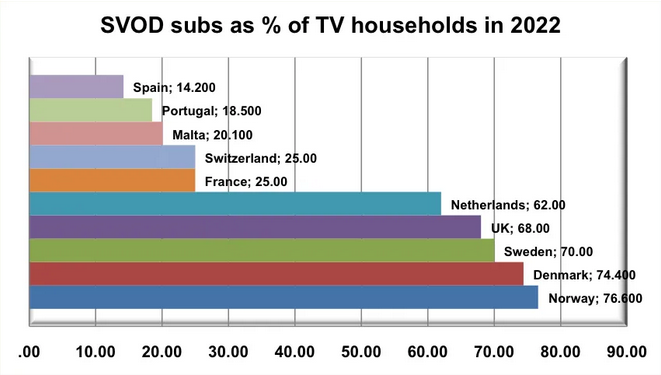
\includegraphics[width=12cm, keepaspectratio]{img/SVoD.png}
			\caption{Estimaciones crecimiento mercado SVoD para Europa Occidental.}
			\label{fig:svod}
		\end{figure}
		
		
		Existen otras muchas plataformas web que ofrecen distintas funcionalidades, por ejemplo: servicio de videoconferencia  en los que destacan Teams y Zoom, repositorios de software como GitHub, plataformas de mensajería instantánea siendo las más utilizadas Whatsapp y WeChat. Cada una de estas plataformas digitales tienen distintas formas de monetizar su servicio, ya sea mediante el uso de \textit{banners} que contengan publicidad, venta de productos en tiendas \textit{online} o sistemas de suscripciones como los usados por muchos periódicos digitales. \\
		
		Gran parte de estas plataformas personalizan la experiencia de uso almacenando y analizando interacciones de sus usuarios para detectar gustos y tendencias. Con esta información logran mostrar unos u otros contenidos y personalizar la publicidad para cada usuario. Un buen ejemplo de esta experiencia personalizada es la que ofrece Youtube en su página principal en la que muestra, basado en el historial de visualizaciones, distintas recomendaciones adaptadas a cada usuario. Con esto se pretende aumentar tanto la satisfacción como la retención de los usuarios.
		
		Con este contexto tan competitivo, disponer de un sistema de monitorización es fundamental en la gestión y administración de cualquier plataforma. Esta necesidad se vuelve crítica cuando la aplicación está desarrollada para ser utilizada por una gran cantidad de usuarios de pago como lo son las aplicaciones web con sistema de suscripciones como Spotify Premium, Twitch Prime o Youtube Premium. La monitorización permite dimensionar mejor la infraestructura de la plataforma, conocer fiablemente el uso que hacen de ella los usuarios y adaptarla mejor a ellos. \\
		
		Estas aplicaciones web hacen uso principalmente información de dos tipos:
		\begin{itemize}
			\item Estructural: contiene datos acerca de los usuarios registrados, permisos de los usuarios y sobre todo información acerca de los contenidos que componen estas secciones ya sean artículos, vídeos, audio, etc.
			
			\item Circunstancial: proporciona información acerca de eventos ocurridos en la aplicación, por ejemplo, las plataformas de vídeo guardarán información acerca de tendencias de visualización para ofrecer recomendaciones más precisas con los gustos de cada usuario. Son los datos que se explotarán en este Trabajo Fin de Grado dentro de la plataforma educativa Kibotics.
		\end{itemize}
		
		Cada usuario que accede a una aplicación espera obtener una experiencia satisfactoria. Por esto, es importante que los contenidos de la aplicación estén diseñados de acuerdo a las necesidades y exigencias de los usuarios. Una forma de comprobar la satisfacción de los usuarios es mediante la monitorización del tiempo invertido en la aplicación y en sus distintas secciones. Para conseguir estos datos es necesario un sistema de monitorización que registre y muestre estos datos. \\
		
		El almacenamiento de estos datos puede ser exponencial por lo que es muy importante tener en cuenta el tipo de base de datos a utilizar para poder tener esta información disponible. A mayor número de usuarios más necesidad de tener una base de datos rápida y eficiente que permita un guardado y consulta masivo de datos. \\
		
		Por otro lado, la consulta manual de los datos almacenados es un proceso tedioso y en muchas ocasiones no garantiza un correcto análisis de los acontecimientos de la plataforma. Para esto, una herramienta que obtenga la información almacenada en la base de datos y la presente en distintas visualizaciones de modo automático y vistoso se convierte en necesaria. Existe una gran variedad de tecnologías dentro de estas herramientas de visualización de datos como, por ejemplo, Cognos Analytics, MongoDB Charts, Metabase... Este TFG se centra en Matplotlib y Kibana.
	
	
	\subsection{Tecnologías web}
	\label{subsec:introduccion_tecnologias_web}	
		
		Este aumento de uso de plataformas digitales, especialmente multimedia, ha sido en parte posible gracias a la salida del estándar HTML 5. Este nuevo estándar ofrece, entre otras mejoras, nuevas características importantes para la transmisión de contenido multimedia con la inserción de la etiqueta vídeo y \textit{canvas} que ofrece la posibilidad incluir vídeos y generar escenas gráficos 2D y 3D de manera nativa. A continuación, se detallan algunas de las principales características del estándar HTML5:
		
		\begin{itemize}
			\item WebGL: API implementada en JavaScript que permite la renderización de gráficos dentro del navegador web. Ofrece aceleración \textit{hardware} haciendo uso de la GPU lo que proporciona un procesamiento y generación de imágenes muy potente.
			\item Webworkers: ofrece la posibilidad de ejecución multihilo en el navegador mediante la creación de \textit{workers} que ejecutan \textit{scripts} en segundo plano, paralelo a la ejecución principal.
			\item WebSockets: Mediante el uso de una API, se hace posible la apertura de comunicaciones interactivas entre el navegador y un servidor. Gracias a un \textit{handshake}, cliente y servidor se conectan permitiendo comunicación bidireccional mediante eventos en la que los mensajes los establece el desarrollador.
			\item WebRTC: Ofrece una API con la que retransmitir audio y vídeo entre navegadores sin necesidad de un intermediario, así como compartir datos y realizar teleconferencias \textit{peer-to-peer}, sin necesidad de complementos o \textit{software} externo.
		\end{itemize}
			
		Gracias a todas estas nuevas herramientas y a \textit{frameworks} web como A-Frame, el cual permite crear escenas 3D e incluso entornos de realidad virtual, las aplicaciones web son cada día más atractivas para las empresas y más potentes para los desarrolladores. \\
		
		Paralelo a estas tecnologías, surgen nuevos entornos de desarrollo web o \textit{frameworks} que ofrecen la posibilidad de crear aplicaciones de forma más rápida. Estas herramientas disponen de capacidades para el desarrollo del lado servidor de una aplicación web como interacciones con bases de datos, cálculos en los servidores, análisis de datos, etc. A continuación se enumeran algunos \textit{frameworks} populares:
		
		\begin{itemize}
			\item Django: \textit{framework} web de alto nivel diseñado para desarrollar servidores en Python.Su filosofía se centra en desarrollos rápidos, limpios y en un diseño pragmático. Sigue el patrón \textit{Model-View-Template} (MVT).
			\item Spring: Diseñado para la creación de aplicaciones Java, ofrece soporte para Groovy y Kotlin. Dispone de una estructura modular y una gran flexibilidad para implementar diferentes tipos de arquitecturas.
			\item NodeJS: Ofrece desarrollo de servidores web basado en JavaScript. Mediante el uso de Websockets consigue ser muy eficiente en aplicaciones de tiempo real.
		\end{itemize}
		
	\section{Robótica educativa}
	\label{sec:1_robotica_edicativa}
		La robótica es una temática transversal, solapándolo con áreas como las matemáticas, tecnología o ingeniería. Centrada en la programación permite desarrollar el pensamiento lógico y la capacidad de solución de problemas. \\
		
		Una posibilidad para iniciarse en el mundo de la robótica es haciendo uso de kits de robótica como los ofrecidos por \texttt{LEGO education}\footnote{https://education.lego.com/es-es} con los que aprender conceptos fundamentales de electrónica y tecnología mediante la construcción de robots y herramientas de codificación en las que proporcionarles diversas funcionalidades. \\
		
		\begin{figure}[H]
			\centering
			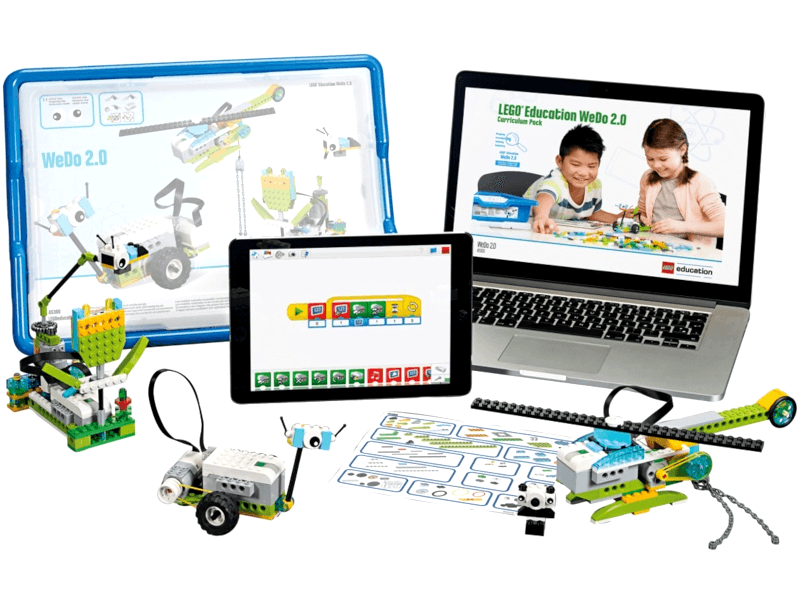
\includegraphics[width=10cm, keepaspectratio]{img/lego.png}
			\caption{Kit de robótica LEGO WeDo 2.0.}
			\label{fig:lego}
		\end{figure}
		
		Estos kits de robótica suelen estar basados en lenguajes de programación como Scratch para implementar el desarrollo de las funcionalidad de los robots. Scratch permite el desarrollo mediante bloques gráficos, ofreciendo así un aprendizaje sencillo sin necesidad de conocimientos previos sobre programación. Gracias a esta característica es una herramienta ideal para que niños aprendan los fundamentos de la lógica y la programación.
		
		\begin{figure}[H]
			\centering
			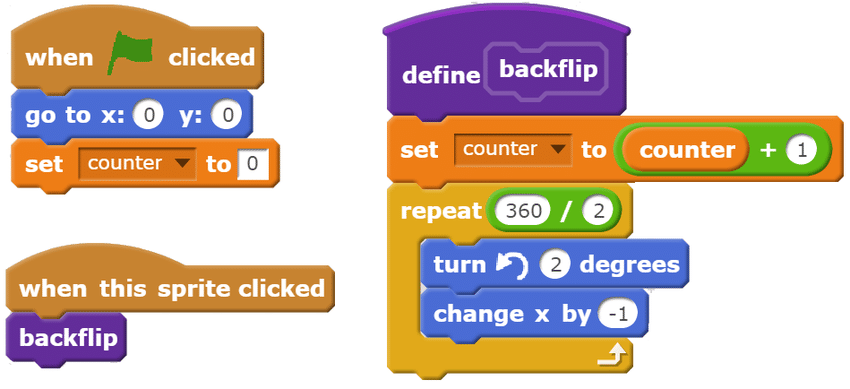
\includegraphics[width=10cm, keepaspectratio]{img/scratch.png}
			\caption{Ejemplo programa de Scratch con tres scripts.}
			\label{fig:scratch}
		\end{figure}
		
		Existen además aplicaciones web que ofrecen un entorno con el que iniciarse en el mundo de la robótica y que, gracias al uso de editores y simuladores \textit{online}, permiten el desarrollo de funcionalidades y la simulación de las mismas sin necesidad de poseer el robot físico. Bajo este contexto, nace en 2016 Open Roberta \footnote{https://lab.open-roberta.org/}, un proyecto educativo con la filosofía \textit{learning with robots} que ofrece un entorno de desarrollo que permite a niños sin conocimientos técnicos previos programar y simular en la web y posteriormente probar en robots como \texttt{LEGO MINDSTORMS}. Open Roberta hace uso de un lenguaje de programación llamado \texttt{NEPO} en el que, siguiendo el paradigma de Scratch, cada bloque representa una funcionalidad del robot ya sea acerca de sensores, acciones o controles. \\
		
		\begin{figure}[H]
			\centering
			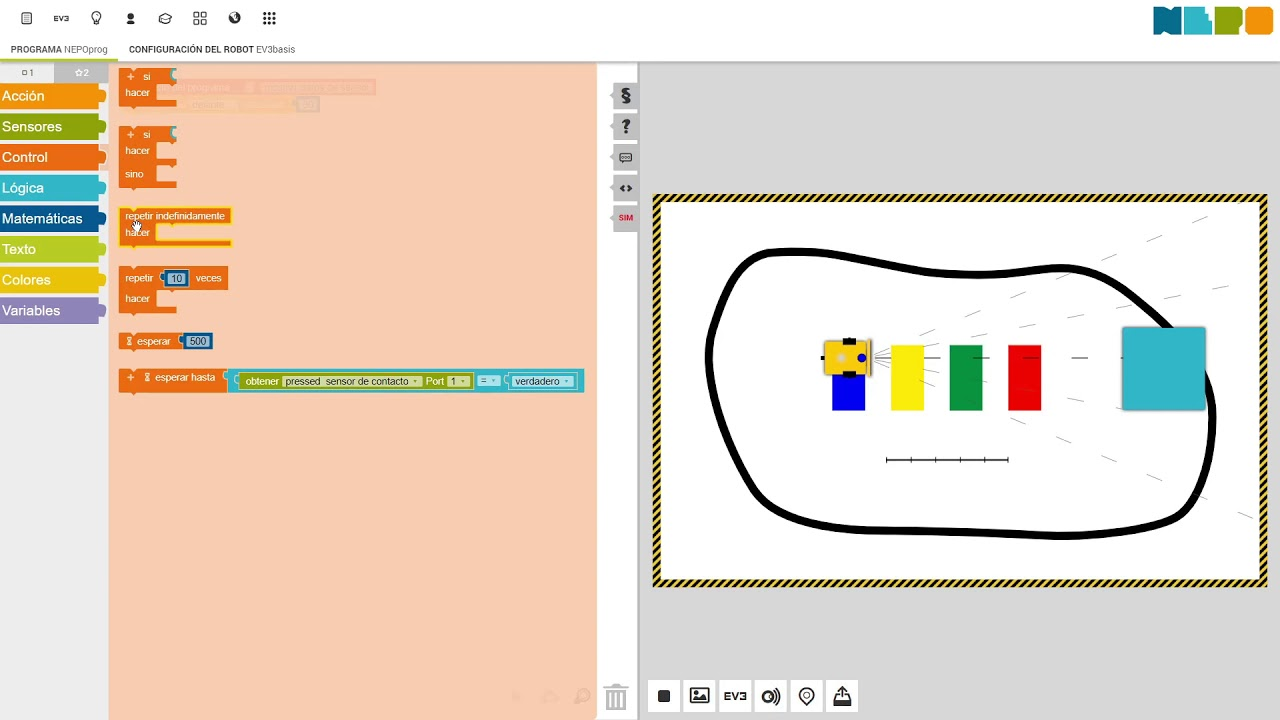
\includegraphics[width=11cm, keepaspectratio]{img/open_roberta.jpg}
			\caption{Editor y simulador Open Roberta.}
			\label{fig:open_roberta}
		\end{figure}
		
		Dentro de este mundo de plataformas educativas \textit{online}, nos centraremos en Kibotics, plataforma en la que se enmarca este proyecto. Ofrece herramientas centradas en la docencia en robótica y programación para alumnos de secundaria. Incluye gran variedad de ejercicios en los que los usuarios pueden aprender conceptos básicos acerca de distintos lenguajes de programación como Scratch o Python, así como introducirse a la visión artificial o la simulación en robots. Kibotics es una plataforma que permite a los usuarios iniciarse en el mundo de la programación de robots, ofrece una gran variedad de ejercicios para que los usuarios se desarrollen en lenguajes como Scratch y Python. Está basada en Django y utiliza A-Frame para la virtualización de los robots.\\
		
		\begin{figure}[H]
			\centering
			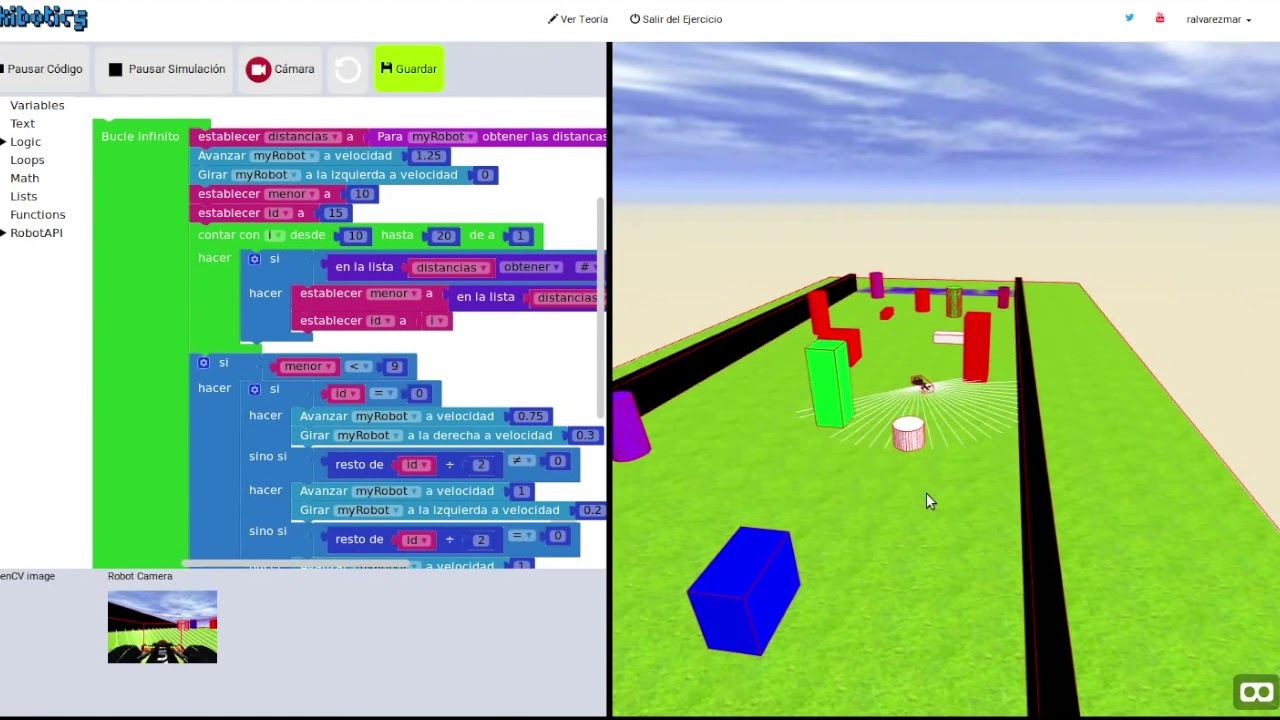
\includegraphics[width=11cm, keepaspectratio]{img/editor_simulador_kibotics.jpg}
			\caption{Editor y simulador Kibotics.}
			\label{fig:editor_simulador_kibotics}
		\end{figure}


	\section{Motivación}
	\label{sec:motivación}
		
		En la plataforma Kibotics los usuarios pueden interactuar de diferentes maneras, el tiempo que le dedican a cada ejercicio puede ser diferente, pueden realizar el mismo ejercicio de diferentes maneras, entran en diferentes horas del día. Conocer las acciones de los usuarios dentro de la plataforma permitiría llevar a cabo acciones de mejora con la intención de aumentar su satisfacción y detectar aquellos elementos que no estuvieran funcionando adecuadamente. Pese a que toda esta información es muy valiosa, actualmente no existe ningún sistema de monitorización para observar qué partes de la plataforma generan más interés y que uso se está haciendo en ella.  \\

		El objetivo de este TFG es dotar a esta plataforma educativa de sondas de almacenamiento de datos y herramientas de visualización para el análisis de éstos, ya sean de visitantes a la web, o usuarios registrados que estén accediendo a ejercicios. De esta manera, se le ofrecería a sus administradores y desarrolladores una solución completa embebida en la web con capacidad para recoger y representar los datos aportados por el uso del servicio para observar su funcionamiento y facilitar la toma de decisiones con el fin de mejorarlo. \\
			
		El diseño de una herramienta de analíticas para una plataforma web no es algo trivial ya que existen diversas tecnologías que podrían ser utilizadas, cada una de ellas con sus ventajas e inconvenientes. De modo que se explorarán varias con el fin de elegir las más adecuadas.
		
		
	\section{Estructura de la memoria}
	\label{sec:1_estructura_memoria}
	La presente memoria se ha ividido en los siguientes capítulos:
	
	\begin{itemize}
		\item En el capítulo \ref{chap:introduccion} se introduce el proyecto ofreciendo el contexto sobre el que se va a trabajar así como la motivación que inició este TFG.
		
		\item En el capítulo \ref{chap:objetivos} se exponen tanto los objetivos a cumplir como la metodología seguida en el transcurso de este proyecto. 
		
		\item En el capítulo \ref{chap:infraestructura_utilizada} se detallan todas las tecnologías involucradas en el desarrollo de este TFG. Se ha dividido en tres secciones: tecnologías Web, bases de datos y tecnologías de visualización. 
		
		\item En el capítulo \ref{chap:primer_prototipo} se define el diseño propuesto para el primer prototipo de la herramienta de analíticas que mejora la funcionalidad de análisis automático en la plataforma Kibotics. Además, se exponen los pasos realizados para el desarrollo e integración del prototipo en producción.
		
		\item En el capítulo \ref{chap:segundo_prototipo} se expone un segundo diseño de la herramienta de analíticas aplicando lo aprendido en el desarrollo del primer prototipo y se detallan los pasos que ha sido necesario realizar en la versión final de la herramienta.
		
		\item En el capítulo \ref{chap:conclusiones} se detallan las conclusiones alcanzadas, así como las competencias adquiridas durante la realización de este proyecto. Además, se plantean futuros trabajos sobre el software desarrollado con los que avanzar hacia una solución más completa.
		
	\end{itemize}
		
		
		
	\cleardoublepage 
	\chapter{Objetivos} 
	\label{chap:objetivos} 
		Una vez establecido el contexto de este Trabajo Fin de Grado, en este capítulo se describirán los objetivos y la metodología empleada.

	\section{Objetivos}
	\label{sec:objetivos}
		El objetivo de este Trabajo Fin de Grado es desarrollar un módulo de analíticas para la monitorización de uso de la plataforma educativa \textit{online} Kibotics. Se pretende que esta herramienta ofrezca a los administradores de la web información sobre aquellos eventos que se consideren importantes mientras los usuarios interactúan con ella. Este objetivo general se ha dividido en varios subobjetivos:
		
		\begin{itemize}
			\item Ampliar el sistema de sondeo para la recogida de datos de uso del servicio dentro del servidor Django de Kibotics. Grabará eventos relevantes como entrada y salida de la plataforma así como acceso a los ejercicios, etc.
			\item Desarrollar el almacenamiento de esta información en una base de datos persistente que permita un guardado masivo de registros y que sea escalable.
			\item Diseñar y desarrollar una visualización web automática dentro de la propia plataforma que proporcione vistas agregadas y tendencias en los datos de uso de la aplicación.
		\end{itemize}
	
		Planteado este objetivo general, es necesaria una fase previa al desarrollo software en la que se estudie y analice Kibotics en su estado actual, tanto la arquitectura utilizada como el sistema de logs existente. Ya con unos conocimientos de la aplicación sobre la que desarrollar, es necesario de un estudio de tecnologías de bases de datos y de visualizaciones existente compatibles con las tecnologías usadas en Kibotics. \\
			
		
	\section{Metodología}
	\label{sec:metodologia}
				
		Para asegurar que se daban los pasos correctos hacia la consecución de este objetivo se ha establecido un plan de reuniones semanales con los tutores del proyecto. En estas se presentaban los progresos de la semana. Además, se han utilizado para resolver dudas y problemas que han ido surgiendo.\\
		
		Se ha seguido el modelo de desarrollo de software por prototipos centrado inicialmente una primera solución de la herramienta creada en varias semanas. Gracias a este primer prototipo, se identificaron requisitos que a priori no se contemplaban y se pudo desarrollar una solución final más completa y eficiente de la herramienta de analíticas web.
		
		Para mantener un control de versiones del código desarrollado,se decidió hacer uso de un repositorio de software. Durante este TFG se han utilizado dos repositorios GitHub. El primero \footnote{https://github.com/RoboticsLabURJC/2019-tfg-angel-perea}, un proyecto personal en el que se han subido periódicamente diferentes recursos como: \textit{scripts}, ficheros de log con los que se trabajó en los momentos iniciales del proyecto, así como pequeñas pruebas sobre servidores Django. \\
		
		Una vez adquirido el contexto y habiendo entendido la forma de trabajar a través de respositorios en GitHub, se comenzó a trabajar en el código integrable en la plataforma. Este código está almacenado en el repositorio privado de Kibotics \footnote{https://github.com/jderobot-hub/kibotics-webserver}. Tras las reuniones semanales, se creaban incidencias en los que se detallaban los problemas y las mejoras a implementar en la plataforma. Estas incidencias han servido como hoja de ruta del trabajo a realizar sobre los que se trabajaba durante la semana. \\
		
		Para permitir que varios desarrolladores pudiesen añadir funcionalidad o solucionar errores de forma paralela, se creaba una nueva rama actualizada con los últimos cambios de la rama principal. Es sobre esta rama sobre la que se desarrollaba la solución a cada incidencia, una vez finalizados los cambios se explicaban en un comentario o \textit{commit} y se subían al repositorio remoto. El siguiente paso consistía en solicitar la fusión de los cambios de esta rama con la rama principal, abriendo peticiones \textit{pull request} (parches). Una vez solicitada la fusión, los desarrolladores responsables, más experimentados, verifican que los cambios son correctos. Si es así, el proceso de integración termina, se fusionan las ramas en la rama maestra oficial y se da por resuelta la incidencia. \\
		
		Durante el desarrollo de este TFG se ha seguido la filosofía \textit{release often, release soon} integrando pequeños cambios semanales gracias al sistema de ramas y parches de Github. Con esta metodología se consiguió que el código a integrar en cada paso no fuese tan extenso, permitiendo a los desarrolladores responsables validar e integrar los cambios más rápido.\\
		
		Se ha usado el dominio gratuito que Github ofrece para crear un blog\footnote{https://roboticslaburjc.github.io/2019-tfg-angel-perea/logbook/}. En este blog se han creado entradas periódicamente en las que se han ilustrado los avances de la herramienta de analíticas.  
		

		
	\cleardoublepage 
	\chapter{Infraestructura utilizada} 
	\label{chap:infraestructura_utilizada} 
		En este capítulo se describen las diferentes tecnologías web, de bases de datos y de visualización que se han utilizado en el transcurso del proyecto.
		
	\section{Tecnologías Web} 
	\label{sec:tecnologias_web} 
		El desarrollo de sitios web o aplicaciones \textit{online} es un ámbito muy amplio con un gran abanico de tecnologías a disposición de los desarrolladores. En esta sección se explorarán las tecnologías web envueltas en el desarrollo del proyecto tanto en el lado cliente como servidor. El la figura \ref{fig:HTML_CSS_JS} se muestran las 3 tecnologías web básicas utilizadas.
		
		\begin{figure}[H]
			\centering
			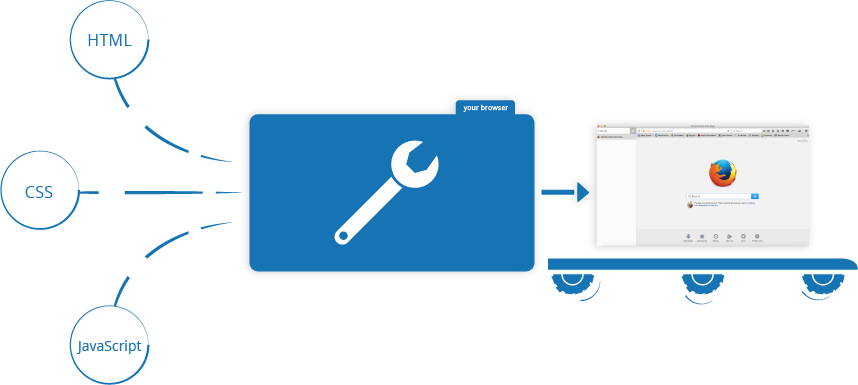
\includegraphics[width=7cm, keepaspectratio]{img/html_css_js.png}
			\caption{Tecnologías web básicas.}
			\label{fig:HTML_CSS_JS}
		\end{figure}
	
	\subsection{HTML}
	\label{subsec:html}
		HTML (Hipertextual Markup Lenguaje) \cite{HTML}, es un lenguaje de marcado. Actualmente utilizado para la definición de  estructura básica de los contenidos de una página web como vídeos, gráficos, texto. \\
		
		Publicado en 1991, su historia se remonta a 1980, cuando Tim Berners-Lee propuso un nuevo sistema para compartir ficheros. Actualmente se ha impuesto como el lenguaje estándar para dar formato a documentos, definido por el \textit{World Wide Web Consortium} (W3C), el cual ha ido evolucionando versión a versión adoptando todas las nuevas exigencias que ofrecen las webs actuales, tanto en el campo de los recursos multimedia como en el de interactividad.\\
		
		HTML se desarrolla haciendo uso de una estructura de etiquetas o \textit{tags}, dentro de las cuales se pueden incluir cada uno de los elementos que conforman una página web. Dispone de cierta capacidad para aportar estilo y lógica pero estas generalmente se delegan en CSS y JavaScript respectivamente.\\
		
		La última versión oficial es HTML5, la cual proporciona soporte nativo para audio y vídeo, inclusión de la etiqueta \texttt{canvas} usada para generar gráficos y efectos tanto en 2D como en 3D, entre otras mejoras. Es la versión usada en este proyecto.
		
	\subsection{CSS}
	\label{subsec:css}
		CSS (Cascade Style Sheet), es un lenguaje de reglas en cascada utilizado para dotar de diseño gráfico a elementos de una página web. Define, como se mencionó anteriormente, la estética de un documento HTML y por lo tanto de una página Web. \\
		
		Permite crear webs atractivas y responsivas, que se adapten al dispositivo en que están siendo vistas, ya sea por ejemplo, tabletas, ordenadores o móviles.\\
		
		Permite mover todas las reglas de estilo (tamaños de fuente o de imágenes, responsividad de elementos a ciertas resoluciones...) a ficheros \texttt{*.css}, evitando así redundancia en un mismo documento \texttt{*.html}, mejorando así la modularidad e independencia dentro de un proyecto.\\
		
		La última versión es CSS3, añade novedades como soporte nativo para transiciones y animaciones. Además de herramientas para una maquetación más precisa. Es la versión usada en este proyecto.
		
	\subsection{JavaScript}
	\label{subsec:javascript}
		JavaScript \cite{JavaScript} es un lenguaje de programación ligero, interpretado, orientado a objetos y dinámico. Utilizado principalmente como lenguaje de \textit{scripting} para paginas web, en este campo su papel principal se centra en el desarrollo de lógica en la parte del cliente \textit{backend}: acceso al \textit{Document Object Model}(DOM) de la web, modificación de etiquetas HTML, generación de gráficos en \textit{canvas} o gestión de \textit{cookies}. \\
		
		Permite crear nuevo contenido dinámico, así como controlar archivos multimedia y gracias al uso de API's (Aplication Programming Interface), enriquece a JavaScript con más funcionalidades permitiendo crear funcionalidades más complejas con desarrollos más simples.
		
	\subsection{Python}
	\label{subsec:python}
		Python es un lenguaje de programación interpretado, orientado a objetos y de alto nivel. Diseñado para un desarrollo de aplicaciones rápido, se utiliza como lenguaje de \textit{scripting} y conexión entre otros componentes de un sistema.\\
		
		Python es simple, con una sintaxis fácil de aprender centrada en la legibilidad del código, consiguiendo así reducir el coste del desarrollo, mantenimiento y ampliación de proyectos.\\
		
		Tiene una gran biblioteca de librerías que puede ser fácilmente extendida por módulos personalizados escritos en C/Python. Haciendo uso del instalador de paquetes \texttt{PIP} (Python Package Installer), es posible la instalación e integración de paquetería en proyectos de manera muy sencilla, así como el cambio de versiones de las mismas.\\
		
		Pese a no ser estrictamente hablando una tecnología web, en este proyecto lo hemos empleado en el contexto de Django, para programar la lógica \textit{backend}. El proyecto comenzó a desarrollarse en Python 2.6 y ha terminado en la versión Python 3.6.9.
		
	\subsection{Django}
	\label{subsec:django}
		Django es un entorno Web de alto nivel diseñado para desarrollar servidores en Python. Al igual que este, su filosofía se centra en desarrollos rápidos, limpios y en un diseño pragmático. Sigue el patrón \textit{Model-View-Template} (MVT) \cite{Django MVC}, donde:
		
		\begin{itemize}
			\item \textit{Model}, esta capa del patrón tiene toda la información relativa a las bases de datos: cómo se almacenan, cómo se relacionan entre ellas, cómo validarlas... Manejado por la capa de bases de datos de Django. Toda esta información de configuración se desarrolla y almacena en el fichero \texttt{Models.py}. Mediante su ORM (Object Relational Model) permite al desarrollador del servidor hacer consultas y manejar los datos de bases de datos relacionales en Python. Los filtros, desarrollados en Python, se traducen automáticamente peticiones \texttt{SQL}.
			
			\item \textit{View}, parte lógica del Framework, se puede ver como una unión entre la capa de modelo y plantillas. Formado por dos ficheros: \texttt{urls.py}, encargado de llamar a la vista adecuada dependiendo de la URL a la que se acceda y \texttt{views.py} con todas esas vistas que devolverán una respuesta HTTP y en las cuales se consultará la capa Model si fuese necesario.
			
			
			\item \textit{Template}, sección que se encargará del qué y cómo mostrar los datos. Manejado por vistas y plantillas de Django que servirán de bases para la parte \textit{frontend} de la Web. Guardado en documentos HTML enriquecidos junto a variables de plantillas Django (\{\{ nombre\_de\_variable \}\}), las cuales permite el uso de, por ejemplo, bucles, operaciones condicionales, diccionarios, inserción de bloques... para generar webs enriquecidas y dinámicas en muy pocas líneas de código.
			
		\end{itemize}


		En la siguiente figura \ref{fig:MTV_Django} se pueden ver gráficamente los ficheros python involucrados en el patrón MVT así como las plantillas HTML enriquecidas que DJango utiliza.
		\begin{figure}[H]
			\centering
			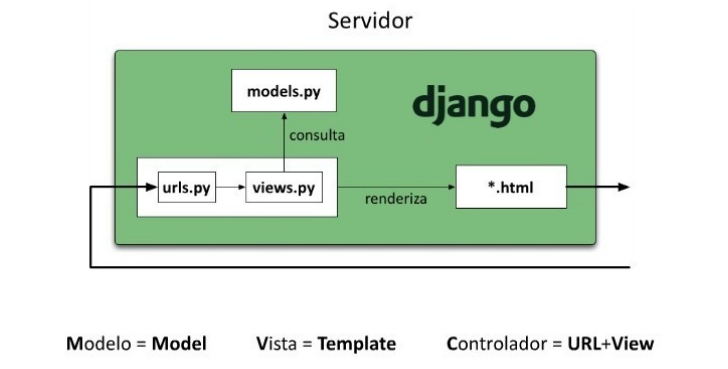
\includegraphics[width=13cm, keepaspectratio]{img/django_MTV.png}
			\caption{Patrón MVT Django.}
			\label{fig:MTV_Django}
		\end{figure}
		
		Diseñado para ser seguro, y evitar errores comunes, Django ofrece una fácil administración de las cuentas de usuarios, así como de sus contraseñas. Además de una sección de administración en la que poder gestionar toda la información almacenada en las bases de datos desplegadas.\\
		
		
		El software ya existente de Kibotics Webserver, servicio web sobre el que se ha trabajado, ya estaba basado en Django. El proyecto comenzó a desarrollarse en la versión 1.9 y ha concluido en la Django 1.11  \cite{Django}.
		
	
	\section{Tecnologías de bases de datos} 
	\label{sec:tecnologias_bases_de_datos} 
		Una base de datos es un conjunto de información, la cual pertenece a un mismo contexto, almacenada de modo sistemático y preservada en distintos formatos, puede ser consultada o alterada posteriormente. En esta sección, se detallarán las distintas tecnologías de bases de datos utilizadas en el desarrollo de este proyecto.
		
	\subsection{MongoDB}
	\label{subsec:mongodb}
		MongoDB \cite{MongoDB} es una base de datos NoSQL (Not only SQL) distribuida, documental (almacenando la información en ficheros BSON, muy similares a JSON), de código abierto y diseñada para ofrecer un nivel productivo alto.\\
		
		Al ser una base de datos NoSQL, permite almacenar información de forma estructurada, pero flexible, pues los esquemas pueden ser cambiados sin necesidad de parar el servicio.
		
		Debido a esta estructura, la velocidad en las consultas es muy alta, convirtiéndose así en una base de datos ideal para trabajar con grandes cantidades de información que vayan a ser consultados muy frecuentemente.\\
		
		La escalabilidad de MongoDB es sencilla, puesto que se ejecuta en \textit{clusters}, podrá escalar horizontalmente contratando más máquinas, aumentando así la capacidad de procesamiento. Es una base de datos muy utilizada en la industria \cite{Use_MongoDB}.\\
		
		Para el primer prototipo de este proyecto, se ha utilizado la última versión estable de MongoDB, la versión 4.2.6.
		
	\subsection{Elasticsearch}
	\label{subsec:elasticsearch}
		Elasticsearch \cite{elasticsearch} es una base de datos. Junto a Logstash y Kibana, los tres proyectos open source, forman el stack ELK. En la siguiente figura \ref{fig:ELK_Stack} se muestra un diagrama de flujo de estas tecnologías involucradas en el stack ELK.\\
		
		\begin{figure}[H]
			\centering
			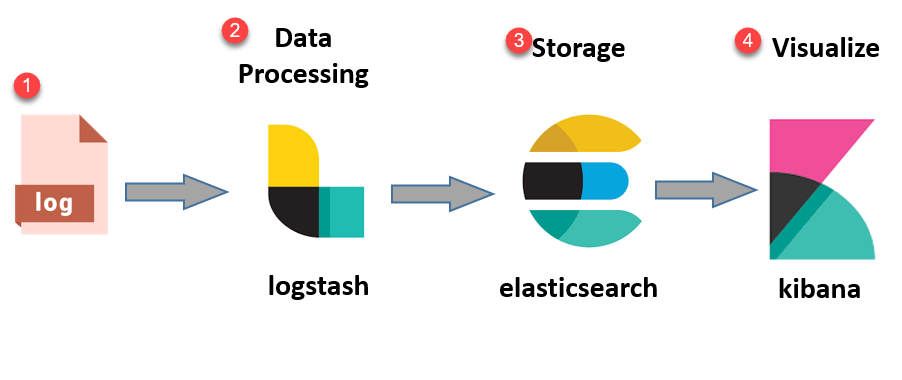
\includegraphics[width=10cm, keepaspectratio]{img/ELK_Stack.png}
			\caption{Stack ELK.}
			\label{fig:ELK_Stack}
		\end{figure}
		
		Basado en Lucene (API para recuperación de información), permite almacenar información compleja como datos de geolocalización así como realizar búsquedas de texto y auto-completado casi en tiempo real. Mediante el uso de una API Rest realiza consultas, borrado y actualización de documentos.\\
		
		En vez de usar filas y columnas, Elasticsearch almacena estructuras complejas de datos serializadas como documentos JSON. Para almacenar estos documentos, Elasticsearch hace uso de índices. Cada uno de estos índices dispone de una estructura de datos propia. Estas estructuras JSON son tambien utilizadas tanto para las consultas y respuestas, lo que la hace sencilla de usar e integrar en sistemas productivos ya existentes.\\
		
		Dadas estas capacidades de almacenar información preparada en índices, la consulta de documentos es muy ágil puesto que evita búsquedas tanto en indices como en documentos no deseados. Organizado en nodos, permitirá aumentar la potencia a medida que la demanda de recursos crezca. \\
		
		Se ha convertido en uno de los buscadores por texto más importantes, utilizado por gigantes de Internet como Facebook, Netflix o Github. \\
		
		La última versión estable de Elasticsearch es la versión 7.8.0 \cite{versions_elasticsearch}, liberada el 18 de Junio del 2020. En proyecto, se ha utilizando la versión 7.6.2 publicada el 31 de Marzo del 2020.
		
	
	\section{Tecnologías de visualización} 
	\label{sec:tecnologias_visualizacion} 
		La muestra de datos es una de las bases de este proyecto, en esta sección se explicarán las tecnologías utilizadas tanto en el primer prototipo como en la versión final del módulo de analíticas desarrollado para este proyecto.
		
	\subsection{Matplotlib}
	\label{subsec:matplotlib}
		Matplotlib es una librería de Python que se encarga de la generación de visualizaciones tanto estáticas como animadas. \\
		
		Proporciona gran variedad de visualizaciones como mapas de calor, gráficas de barras, histogramas... recordando a Matlab. Ofrece cierta capacidad de estilo y puede ser utilizada junto a otras librerías para generar visualizaciones aún más complejas y enriquecidas como mapas geográficos en los que se representa datos mediante latitud y longitud. \\
		
		En la siguiente figura \ref{fig:visualizations_matplotlib} se muestran unos ejemplos de diferentes tipos de visualizaciones que Matplotlib ofrece.
		\begin{figure}[H]
			\centering
			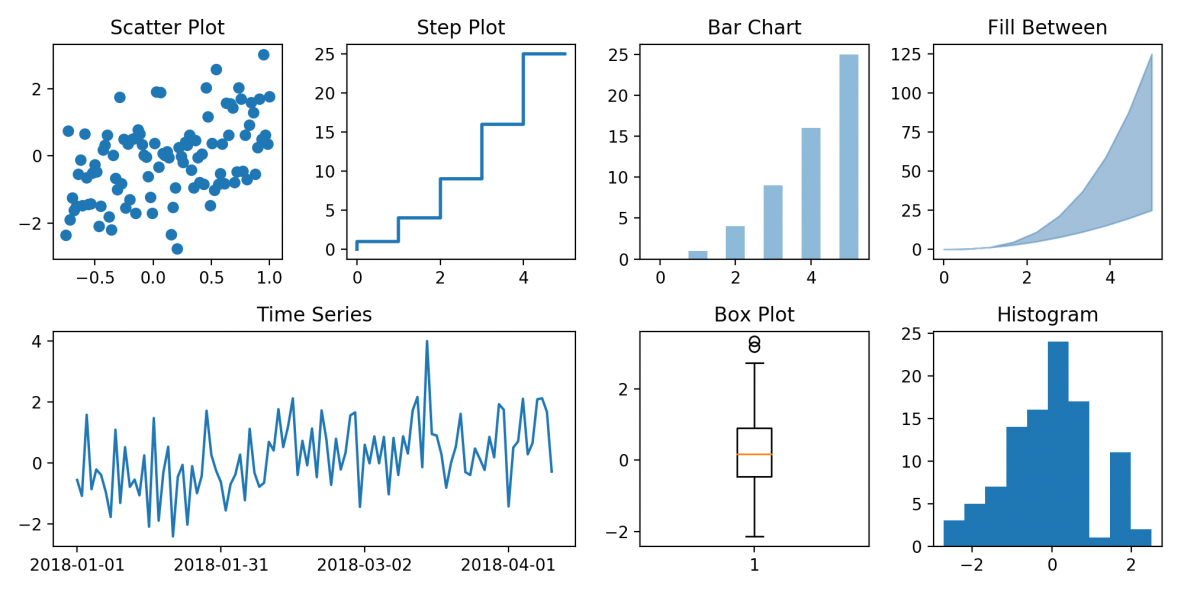
\includegraphics[width=11cm, keepaspectratio]{img/visualizations_matplotlib.png}
			\caption{Visualizaciones en Matplotlib.}
			\label{fig:visualizations_matplotlib}
		\end{figure}
		
		Matplotlib almacena las visualizaciones en figuras, cada una contiene los ejes en que se representarán los datos, estos ejes pueden ser de múltiples tipos, ya sean coordenadas x-y, x-y-x para una representación en tres dimensiones o un eje polar.\\
		
		Las visualizaciones generadas podrán ser mostradas en una nueva ventana si utilizamos la librería en un \textit{script} o ser renderizadas y devueltas como imagen \texttt{PNG} para su posterior muestra en el servicio web haciendo uso de la etiqueta \texttt{HTML} <img></img>\\
		
		En el primer prototipo de este proyecto se utilizó la versión 3.1.2 de Matplotlib, publicada el 18 de Marzo del 2020 \cite{releases_matplotlib}.
		
	\subsection{Kibana}
	\label{subsec:kibana}
		Como se comentó anteriormente, el stack ELK está compuesto por Kibana \cite{kibana} como motor de búsqueda, procesador de datos y generador de visualizaciones entre otras funcionalidades. Diseñada para utilizar Elasticsearch como fuente de datos.\\
		
		Gracias a su aplicación \textit{frontend}, la creación de visualizaciones se simplifica mucho sin ser necesaria la codificación de estas. \\
		
		Mediante configuración, filtrado y selección de los datos indexados en Elasticsearch se pueden crear múltiples tipos de visualizaciones interactivas (gráficos de barras,  circulares, tablas, histogramas y mapas), y posteriormente ser agrupadas en tableros o \textit{Dashboards}, los cuales permiten la visualización y posterior filtrado de grandes cantidades de información de forma simultanea y sencilla.\\
		
		En la siguiente figura \ref{fig:visualizations_kibana} se muestran unos ejemplos de diferentes tipos de visualizaciones que Kibana ofrece.
		
		\begin{figure}[H]
			\centering
			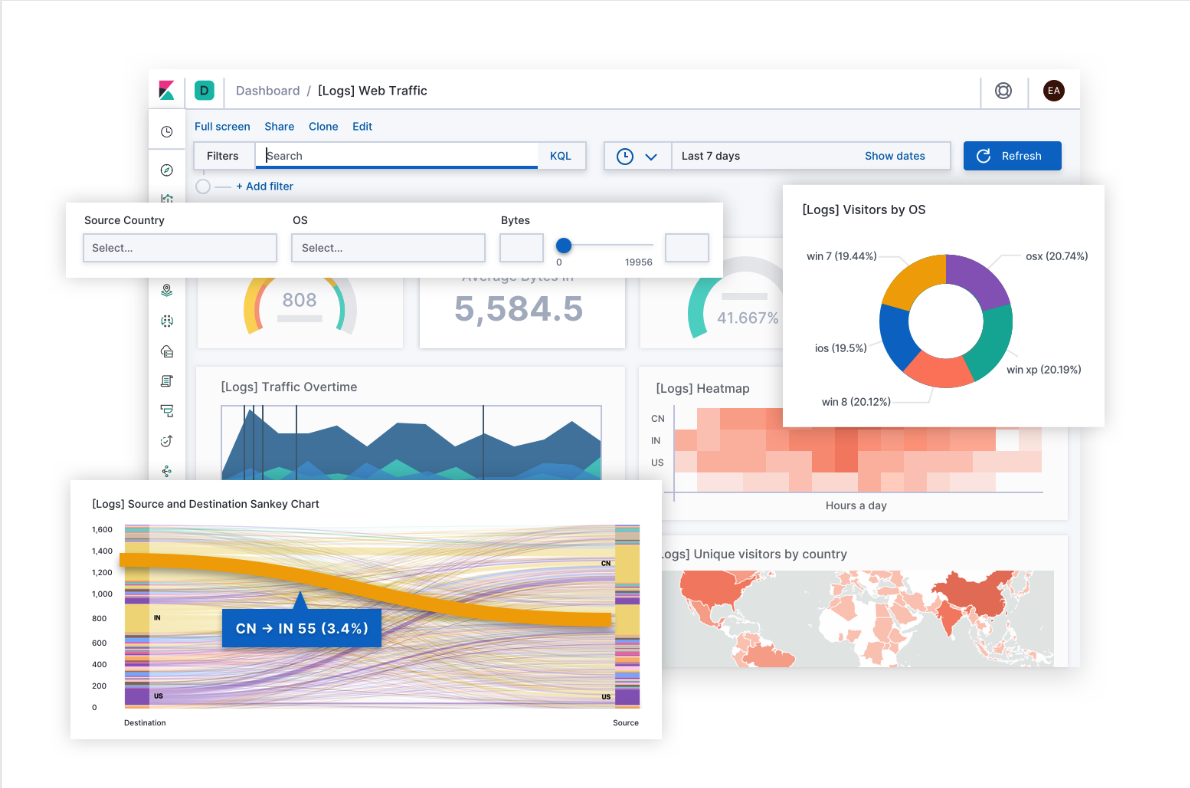
\includegraphics[width=12cm, keepaspectratio]{img/visualizations_kibana.png}
			\caption{Visualizaciones en Kibana.}
			\label{fig:visualizations_kibana}
		\end{figure}
		
		Permite el procesado de los documentos ya indexados en Elasticsearch para crear nuevos campos dinámicos que podrán ser utilizados y representados posteriormente en visualizaciones y estadísticas.\\
		
		Ofrece una interfaz segura y organizada, dividida en espacios de trabajo o \textit{spaces} como se muestra en la figura \ref{fig:spaces_kibana}. Estos espacios pueden ser tratados como instalaciones de Kibana independientes permitiendo a varios equipos de trabajo hacer uso del mismo servicio de Kibana sin los inconvenientes de compartir información de índices. Aumentando la compartimentalización y escalabilidad del servicio.
		
		
		\begin{figure}[H]
			\centering
			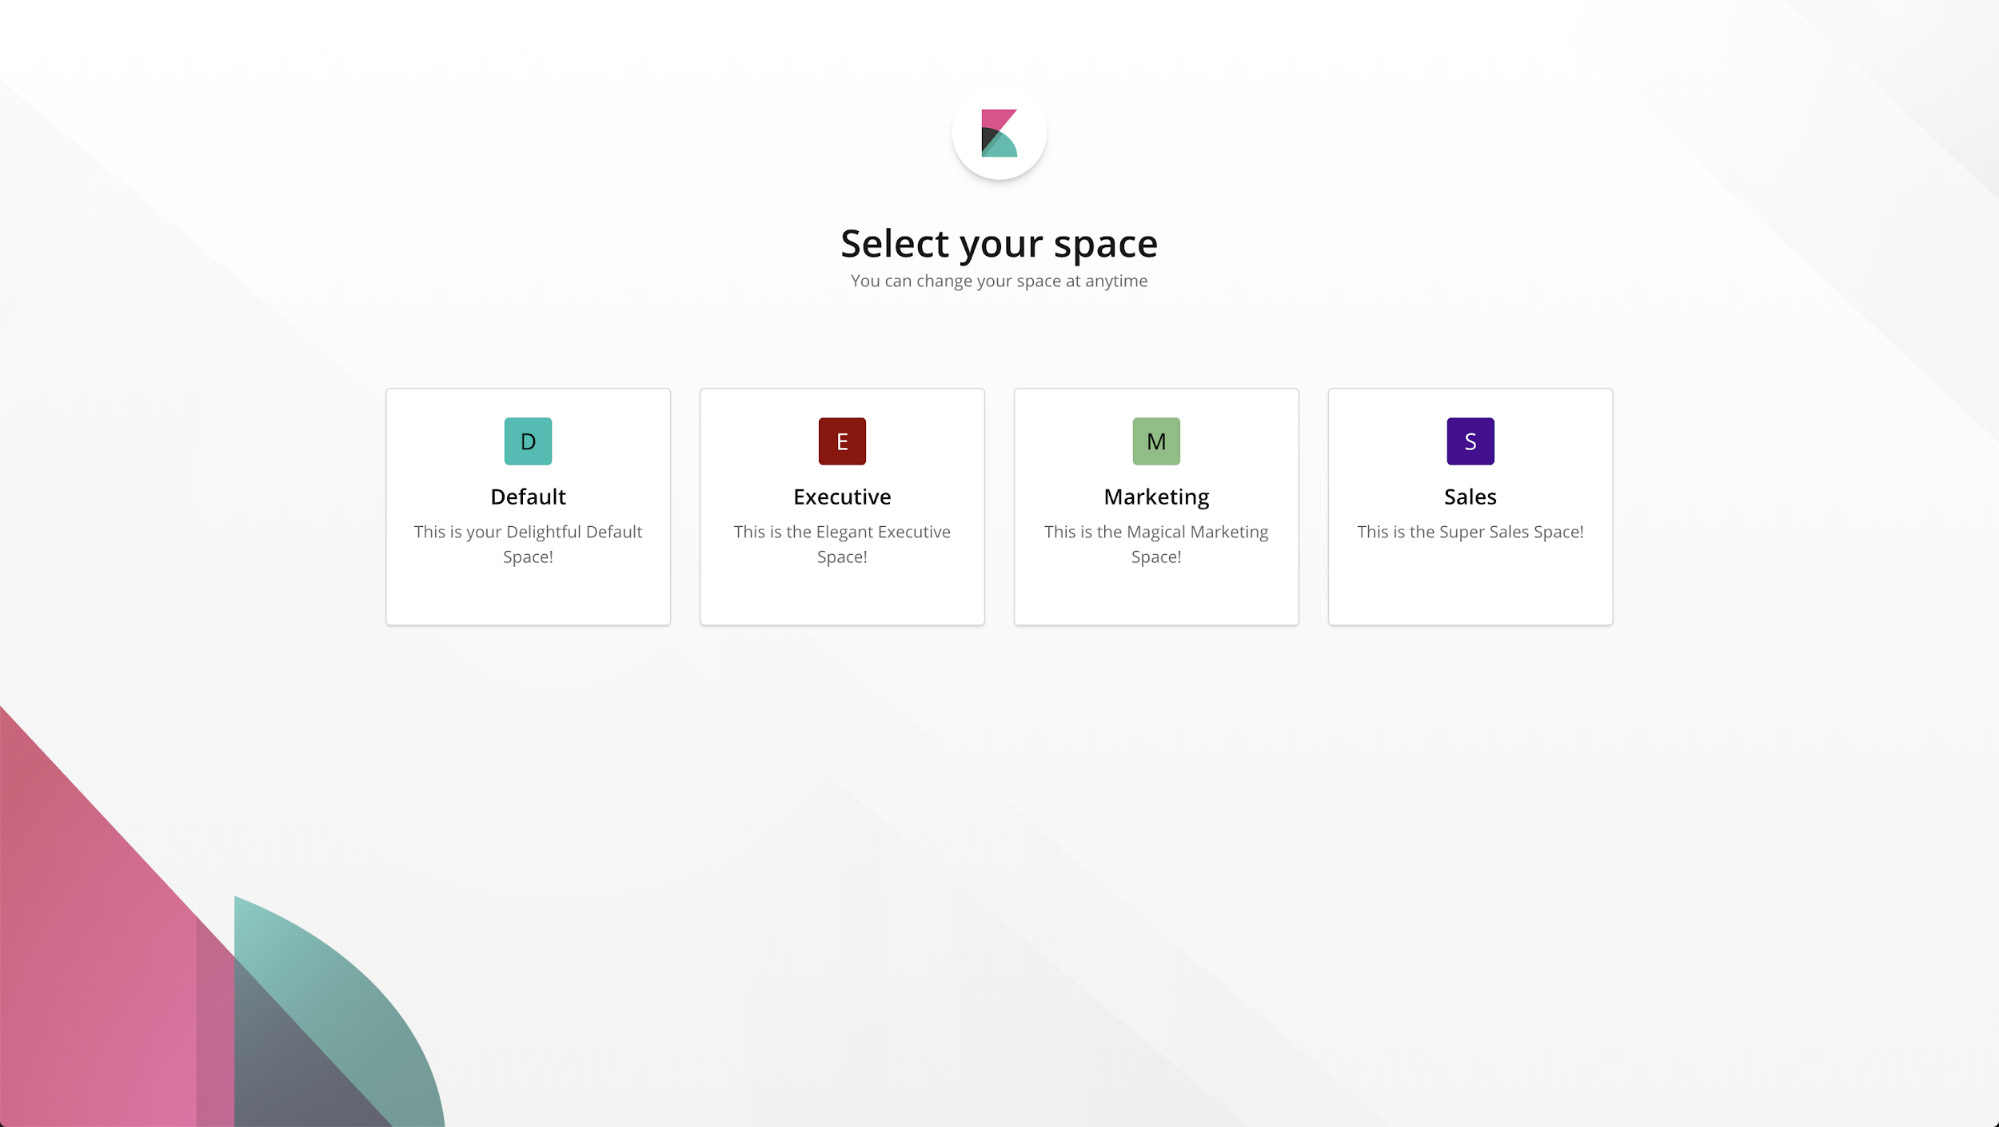
\includegraphics[width=12cm, keepaspectratio]{img/spaces_kibana.jpg}
			\caption{Selector de espacios de trabajo en Kibana.}
			\label{fig:spaces_kibana}
		\end{figure}
		
		La última versión estable de Kibana es la 7.8.0 \cite{versions_kibana}, liberada el 18 de Junio del 2020. En la versión final desarrollada se ha utilizado Kibana 7.7.0 publicada el 13 de Mayo del 2020.
	
	

	\cleardoublepage 
	\chapter{Analíticas basadas en MongoDB y Matplotlib} 
	\label{chap:primer_prototipo} 
		En este capítulo se describe el estado inicial de la plataforma Kibotics en cuanto a recogida automática de datos y su análisis, tanto arquitectura de la aplicación como las tecnologías en las que está desarrollado. Además, se define el diseño que se ha implementado en el primer prototipo que mejora la funcionalidad de análisis automático en la plataforma Kibotics. Se exponen los pasos realizados para la integración de MongoDB como base de datos, y de Matplotlib como generador de visualizaciones de la herramienta de analíticas que se integrará en Kibotics Webserver.
	
	
	\section{Antecedentes} 
	\label{sec:1_antecedentes} 
		Kibotics es una plataforma educativa \textit{online}, en la que se enmarca este proyecto. Ofrece herramientas centradas en la docencia en robótica y programación para alumnos de secundaria. Con una gran variedad de ejercicios en los que los alumnos pueden aprender conceptos básicos acerca de distintos lenguajes de programación como Scratch o Python, así como introducirse a la visión artificial o la simulación en robots. Estos ejercicios tienen dos secciones principales:
		
		
		\begin{enumerate}
			\item Una primera vista con contenidos teóricos, incluye una explicación del ejercicio así como conceptos útiles en la resolución del mismo. 
			\item La segunda vista es donde los alumnos desarrollen su solución. Dividida en el editor y en el simulador \texttt{WebSim}, como se muestra en la Figura \ref{fig:editor_simulador_kibotics}. El simulador web ejecuta el código desarrollado en el editor de texto.
		\end{enumerate}
		
		\begin{figure}[H]
			\centering
			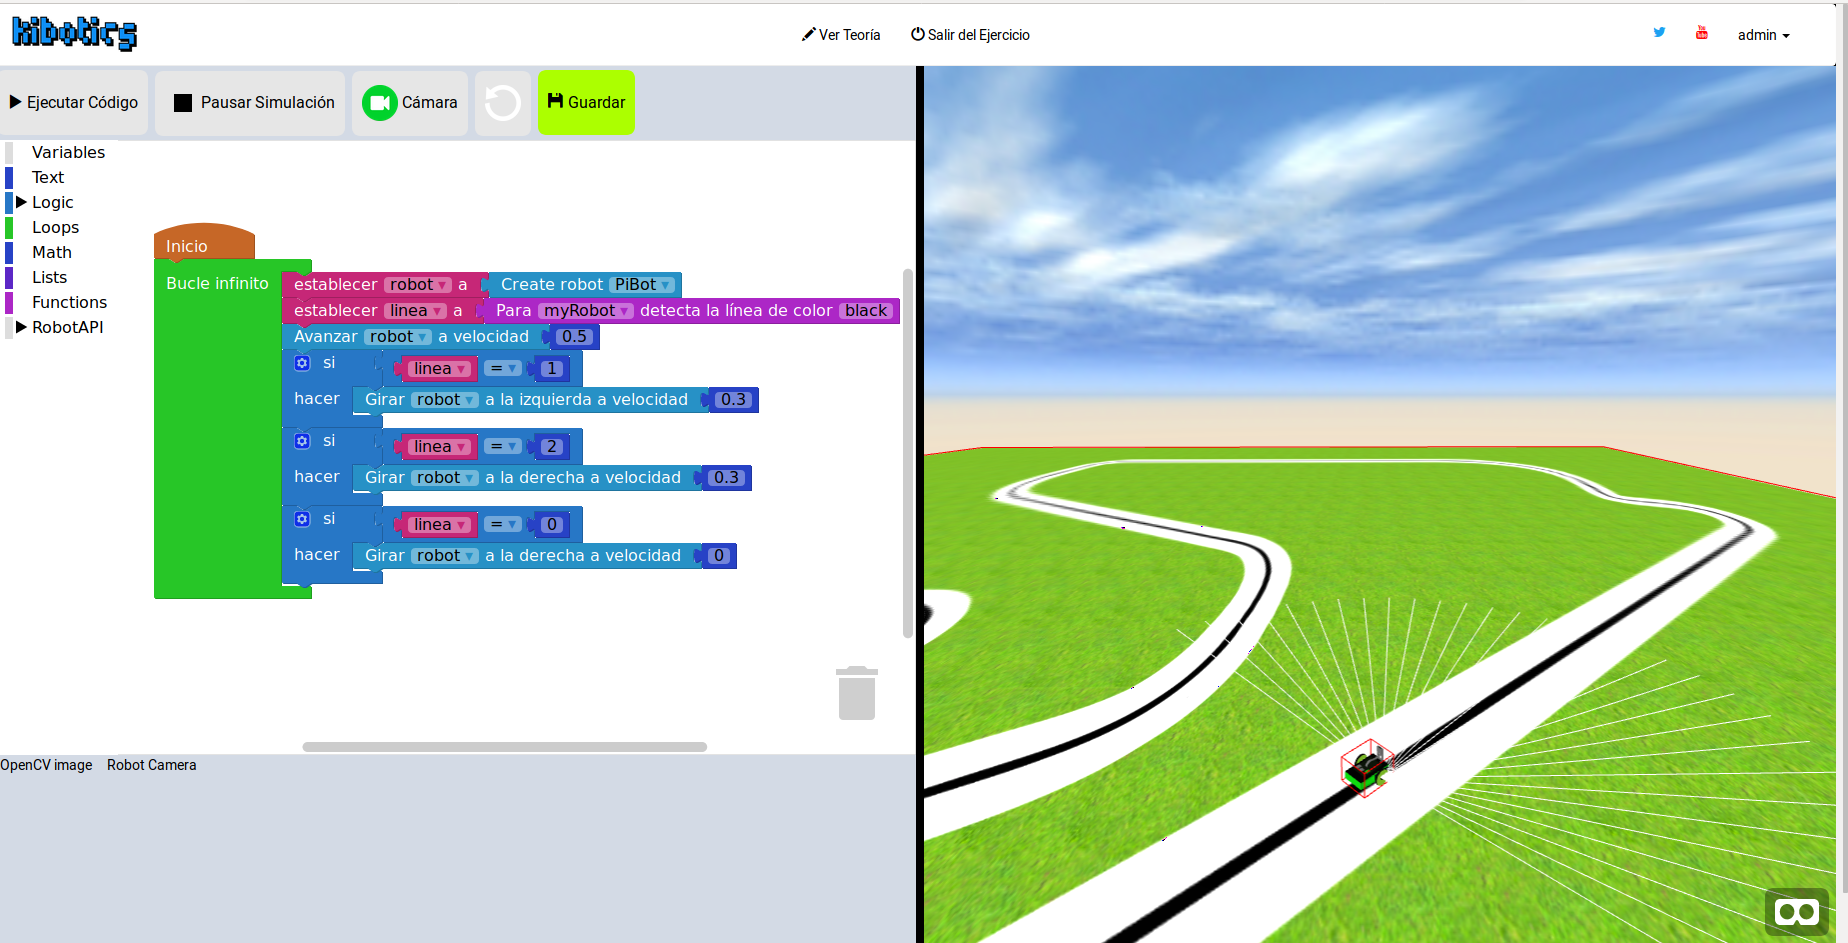
\includegraphics[width=13cm, keepaspectratio]{img/websim-siguelinea.png}
			\caption{Editor y simulador en Kibotics.}
			\label{fig:editor_simulador_kibotics}
		\end{figure}
		
		Una vez resuelto el ejercicio, Kibotics genera un fichero con la solución que el usuario puede descargar para probarlo en un robot real. En el siguiente enlace se muestra un vídeo de un robot sobre el que se ha cargado código desarrollado en Kibotics. \footnote{\url{https://www.youtube.com/watch?v=a0aIqyyEEnw}} \\
		
		Kibotics es un servicio web complejo y compuesto de muchas tecnologías distintas. La Figura \ref{fig:arquitectura_kibotics} muestra la arquitectura que poseía Kibotics 2.0 inicialmente, en ella podemos observar:
		
		\begin{itemize}
			\item Webserver: Servidor web desarrollado en Django, es el centro de Kibotics y donde se generan los logs sobre los que se trabaja en este Trabajo Fin de Grado. Se apoya en una base de datos MySQL para almacenar todos los datos de información estructural de la aplicación y en unos ficheros de log \texttt{*.txt} en los que se almacena información circunstancial de uso de la aplicación.
						
			\item Websim: Simulador robótico que se ejecuta únicamente en el lado del cliente. Desarrollado en A-Frame, HTML5, JavaScript. Permite a los usuarios aprender los fundamentos de la programación robótica y visión artificial.
		\end{itemize}
		
		\begin{figure}[H]
			\centering
			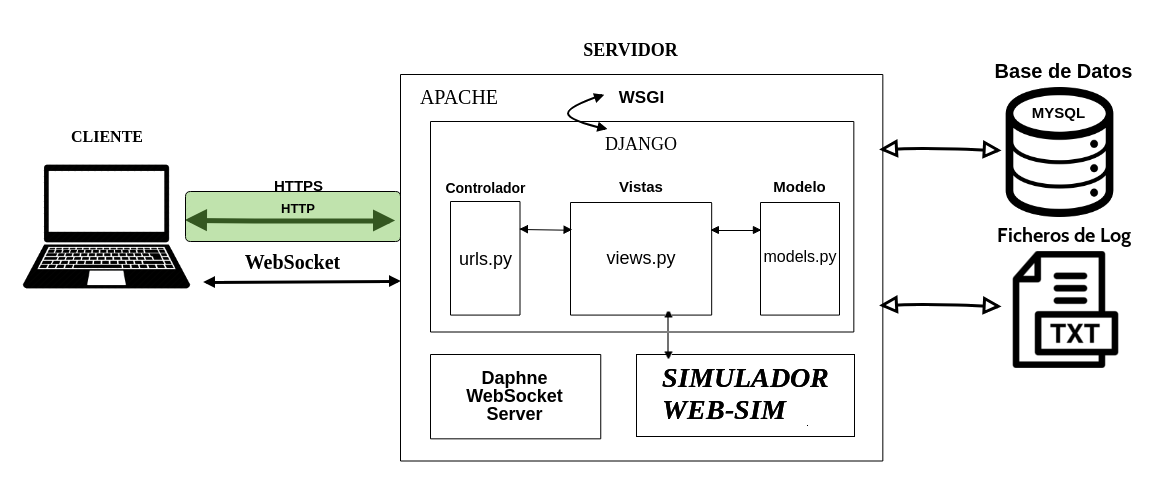
\includegraphics[width=15cm, keepaspectratio]{img/esquema_Kibotics.png}
			\caption{Arquitectura Kibotics.}
			\label{fig:arquitectura_kibotics}
		\end{figure}
		
		Kibotics 2.0 necesita de datos para ofrecer su servicio, estos datos se pueden dividir en dos tipologías:
		\begin{itemize}
			\item Estructurales: almacenados en la base de datos MySQL, ofrecen información acerca de los usuarios registrados, ejercicios de la aplicación, permisos de acceso a estos ejercicios, etc.
			
			\item Circunstanciales: guardados inicialmente en ficheros de texto, proporcionan información acerca de eventos ocurridos en la aplicación por los usuarios como inicio de sesión, fin de sesión, inicio de un ejercicio o salida de un ejercicio. Son los datos que se explotarán en este Trabajo Fin de Grado.
		\end{itemize}
		
		Los datos circunstanciales o logs generados por la aplicación Django se guardan en una serie de archivos indexados en el servidor con formato \texttt{yyyy-MM-dd-log.txt}. Teniendo así un fichero por día con todos los eventos registrados.\\
		
		Inicialmente Kibotics almacenaba 5 eventos distintos: entrada a la plataforma, salida de la plataforma, comienzo de ejercicio, fin de ejercicio y error genérico de la aplicación. \\
		
		Esta metodología de registro de datos circunstanciales disponía de un sistema numeral de códigos para identificar el evento que había generado cada registro de log. Cada uno de estos registros estaba separado por la cadena de caracteres: "\ |\ ". Estos códigos numéricos y su estructura son los siguientes:
		
		\begin{itemize}
			\item Log in: "1 | date | user name | user IP | HTTP\_USER\_AGENT"
			\item Log out: "2 | date | user name | user IP | HTTP\_USER\_AGENT"
			\item Comienzo ejercicio: "3 | date | user name | user IP | simulation type | exercise ID | host IP | HTTP\_USER\_AGENT"
			\item Fin ejercicio: "4 | date | user name | user IP | simulation type | exercise ID | host IP | HTTP\_USER\_AGENT"
			\item Error 500: "5 | 500 Internal Server Error"
		\end{itemize}
		
		Estos eventos logueados se generaban en el servidor Django haciendo uso de sondas programadas en Python, las cuales registran el evento en distintas partes del código del servidor web para guardarlas en los ficheros. Un ejemplo de estas sondas para el registro de un evento de \textit{log in} es:
		{\footnotesize
		\begin{verbatim}
			log = open(DIRECTORY + "/logs/" + str(date.today()) + "-log.txt", "a")
			
			traze = "1 | " + str(datetime.now().strftime("%d/%m/%Y %H:%M:%S")) 
			+ " | " + username + " | " + client\_ip  + " | " + user\_agent + "\\n"
			
			log.write(traze)
			
			log.close()	
		\end{verbatim}
		}
	
		Además de estos logs generados en Django, se disponía de los generados de forma automática por Apache. Apache separa los eventos registrados en dos ficheros:  
		\begin{itemize}
			\item Un archivo con la salida general de la aplicación, asociada a los \textit{prints} y excepciones producidas en el servidor.
			\item Un archivo de acceso al servidor que muestra las peticiones \texttt{HTTP} que este ha recibido.
		\end{itemize}
		
		Inicialmente en Kibotics 2.0 no se explotaban estos ficheros de log extraídos del servicio Django, simplemente se almacenaban sistemáticamente en el servidor y se consultaban a mano si la ocasión lo requería.
		
		
		
	\section{Diseño} 
	\label{sec:1_diseno} 
%		en vez de grabar en fichero, grabar en mongoDB -> PORQ!
%		explicar el porque del elegir a MATPLOTLIB
%		
%		sobre el dibujo anterior de la arquitectura añadir las nuevas sondas, así como la base de datos
%			- vistas de análisis

		Para el desarrollo de este primer prototipo de la herramienta de análisis integrada en Kibotics el primer paso es realizar un diseño con las tecnologías a usar. \\
		
		Kibotics Webserver disponía de una tecnología primitiva de trazabilidad de logs basada en ficheros \texttt{TXT} con eventos limitados. La apertura y cierre constante de estos ficheros acarrea un gran coste computacional, limitando así la explotación masiva de estos datos para la generación de estadísticas útiles.\\
		
		Kibotics es una plataforma digital que pretende dar servicio a una gran cantidad de usuarios. Por lo tanto, se espera que la capacidad de procesamiento, almacenamiento y consulta de los logs aumente. Haciendo uso de ficheros de texto plano no se podrá conseguir la velocidad de procesamiento necesaria. \\
		
		Es por esto, por lo que en un primer prototipo se decidió cambiar a un motor de bases de datos para los datos circunstanciales. Se ha decidido explorar MongoBD, es una base de datos NoSQL que permite almacenar información de forma estructurada tal y como se vio en el capítulo \ref{chap:infraestructura_utilizada}. Debido a esto, la velocidad en las consultas es muy alta aún con gran cantidad de datos. Ya que se espera almacenar información de forma masiva, MongoDB es una buena opción para la herramienta de análisis a desarrollar en este primer prototipo. \\

		Para que Kibotics almacene la información de eventos será necesario modificar las sondas ya existentes en Kibotics Webserver que almacenaban información en ficheros de texto plano \texttt{TXT} para que guarden los datos en MongoDB. Además, se ampliará el número de eventos de los que se guarda información en la base de datos circunstanciales. \\
		
		En este primer prototipo además se desarrollará e incorporará a la plataforma la capacidad de visualización de los datos circunstanciales generados, vistos de manera agregada. Para visualizar estos datos almacenados se usará Matplotlib. Es una librería de Python por lo tanto la integración en Django será simple, se desarrollará toda la funcionalidad en un fichero Python llamado \texttt{analitycs.py} y se creará una vista específica de Django para mostrar esas visualizaciones. Es a este al que Django accederá para la generación de las visualizaciones que posteriormente se enviarán a las plantillas HTML enriquecidas de Django. \\
		
		En la Figura \ref{fig:arquitectura_kibotics_1} se muestra de forma esquemática los cambios que se han explorado en este primer prototipo en Kibotics Webserver, tanto el cambio en las sondas para almacenar los datos de log en MongoDB como el uso de Matplotlib como herramienta principal de generación de visualizaciones automáticas.

		\begin{figure}[H]
			\centering
			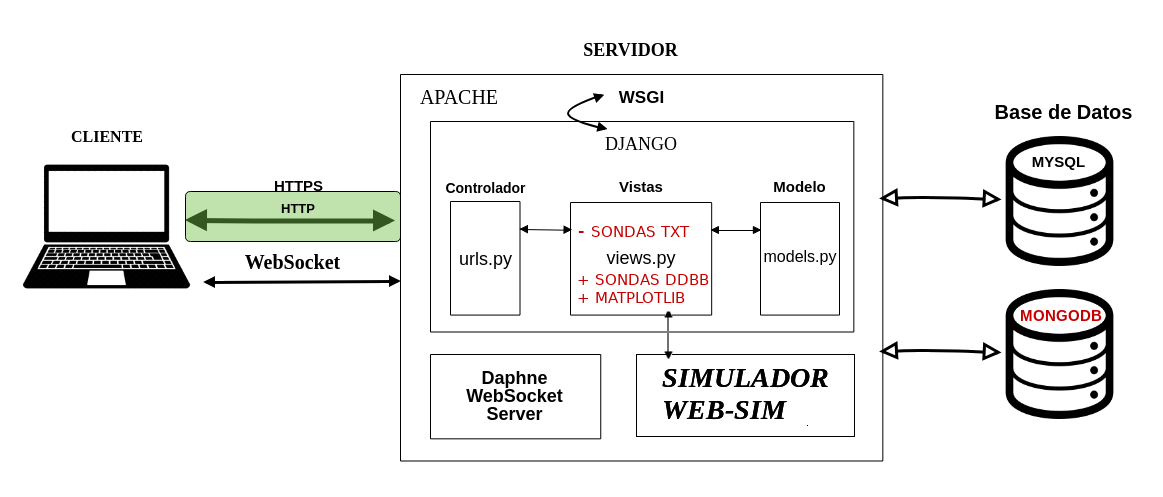
\includegraphics[width=15cm, keepaspectratio]{img/esquema_Kibotics_1.png}
			\caption{Arquitectura Kibotics con funcionalidad de analíticas mejorada usando MongoDB y una vista de datos agregados basada en Matplotlib.}
			\label{fig:arquitectura_kibotics_1}
		\end{figure}

	
	\section{Implementación} 
	\label{sec:1_implementacion} 
		En esta sección se detallan los pasos que ha sido necesario realizar para el desarrollo software del primer prototipo de la herramienta de análisis integrada en Kibotics. Se divide en la integración de MongoDB como base de datos NoSQL de logs y de Matplotlib como generador de visualizaciones. 
		
	\subsection{MongoDB en Webserver}
	\label{subsec:mongodb_kibotics}
		Para la integración de MongoDB en Kibotics Webserver primero se realizó una instalación local del servicio MongoDB para verificar la viabilidad de la tecnología en este primer prototipo. Para ello se ejecuta la siguiente sentencia:
		
		{\footnotesize
		\begin{verbatim}
			$ sudo apt-get install mongodb-org
		\end{verbatim}
		}
		
		Una vez instalado, se levanta el servicio MongoDB:
		
		{\footnotesize
		\begin{verbatim}
			$ sudo systemctl start mongod
		\end{verbatim}
		}
	
		Adicionalmente a esto, podemos reiniciar o parar el servicio con las siguientes sentencias respectivamente:
		
		{\footnotesize
		\begin{verbatim}
			$ sudo systemctl restart mongod
			$ sudo systemctl stop mongod
		\end{verbatim}
		}
	
		Con la base de datos MongoDB ya instalada y configurada el siguiente paso es migrar las sondas previamente definidas. Estas sondas, pasarán de escribir en ficheros a registrar los eventos en MongoDB. \\
		
		Haciendo uso de la librería \texttt{pymongo} para comunicarnos con la base de datos, la tarea se simplifica mucho. Primero importamos la librería y abrimos la conexión con la base de datos, para ello: 
		
		{\footnotesize
		\begin{verbatim}
			import pymongo
			myclient = pymongo.MongoClient("mongodb://localhost:27017/")
			mydb = myclient["kiboticsDDBB"]
		\end{verbatim}
		}
	
		Ya con las conexiones necesarias realizadas, como se puede observar en el siguiente código Python, cada una de las sondas almacenará la información de log en una tabla distinta. Las sondas se transforman a, por ejemplo, las de nueva sesión y nueva simulación:
		
		{\footnotesize
		\begin{verbatim}
			# Nueva sesión
			mydict = {
			    "date" : datetime_object_test, 
			    "username" : "USERNAME_TEST", 
			    "client_ip" : "CLIENT_IP_TEST", 
			    "user_agent" : "USER_AGENT_TEST"
			}
			mydb["newSession"].insert_one(mydict)
			
			# Nueva simulación
			mydict = {
			    "date" : datetime_object_test, 
			    "username" : "USERNAME_TEST", 
			    "client_ip" : "CLIENT_IP_TEST", 
			    "simulation_type" : "SIMULATION_TYPE_TEST",
			    "exercise_id" : "EXERCISE_ID_TEST",
			    "host_ip" : "HOST_IP_TEST",
			    "container_id" : "CONTAINER_ID_TEST",
			    "user_agent" : "USER_AGENT_TEST"
			}
			mydb["newSimulation"].insert_one(mydict)
		\end{verbatim}
		}
		
		Con estos pasos, el registro de eventos de log en la nueva base de datos MongoDB ya está completo. Para recuperar la información y tratarla en el servidor se hará uso, una vez más, de \texttt{pymongo}. Las sentencias o \textit{queries} de búsqueda para los diferentes eventos logueados serán:
		
		
		{\footnotesize
		\begin{verbatim}
			# Sentencia nueva sesión
			dataNSES = mydb["newSession"].find({
			    "username" : {'$regex' : "USERNAME_TEST"}, 
			    "date" : {'$lte': first_day_test, '$gte': last_day_test}
			});
			
			# Sentencia fin de sesión    
			dataESES = mydb["endSession"].find({
			    "username" : {'$regex' : "USERNAME_TEST"}, 
			    "date" : {'$lte': first_day_test, '$gte': last_day_test}
			});
			
			# Sentencia nueva simulación
			dataNSIM = mydb["newSimulation"].find({
			    "username" : {'$regex' : "USERNAME_TEST"}, 
			    "date" : {'$lte': first_day_test, '$gte': last_day_test}
			});
			
			# Sentencia fin de simulación
			dataESIM = mydb["endSimulation"].find({
			    "username" : {'$regex' : "USERNAME_TEST"},
			    "date" : {'$lte': first_day_test, '$gte': last_day_test}
			});
		\end{verbatim}	
		}
	
		Como se puede observar, estas sentencias de búsqueda filtran tanto por usuarios como por rangos de fechas. Esto aporta cierta flexibilidad en la obtención de los eventos, evitando así tener que recorrer datos o ficheros extra descartando registros de log, como se haría con la metodología de ficheros que poseía Kibotics inicialmente.
	
	
	\subsection{Matplotlib en Webserver}
	\label{subsec:matplotlib_kibotics}
		Matplotlib es una librería Python de generación de visualizaciones tanto estáticas como animadas tal y como se presentó en el capítulo \ref{chap:infraestructura_utilizada}. Haciendo uso de ella, se han generado todas las visualizaciones necesarias para el primer prototipo de este Trabajo Fin de Grado.\\
		
		Estas visualizaciones inicialmente se han separado en dos secciones, analíticas de simulaciones y analíticas de sesiones. Ambas pueden ser filtradas tanto por usuarios como por rangos de fechas.\\
		
		Siguiendo la metodología detallada en las secciones anteriores surgió un problema, los datos de inicio y fin, tanto para las sesiones como para las simulaciones, están separados en distintas tablas de MongoDB. Por lo tanto, para relacionar ambos eventos es necesario cruzarlos en Python para unificarlos en un único evento de sesión o simulación. \\
		
		Para solventar esta problemática se desarrolló un método con esta funcionalidad de unificación de registros, con el que se consigue extraer información valiosa de duración de eventos:
		
		Este código fuente extrae todos los usuarios contenidos en el campo \texttt{username} y posteriormente recorre los registros de apertura de cada uno de ellos. Buscando por el campo \texttt{date} de los eventos de cierre hasta encontrar la inmediatamente posterior que será almacenado junto con la duración del evento. \\
		
		Como salida del método, se devolverá un diccionario de diccionarios con cada uno de los eventos de sesión/simulación para cada usuario del que haya ocurrencias.\\
		
		{\footnotesize
		\begin{verbatim}
		
			def formatDatesUser(newData, endData):
			
			    users = newData.distinct("username")
			    newData.sort([('Username', -1), ('date', -1)])
			    endData.sort([('Username', -1), ('date', -1)])
			    Dict = {}
			
			    for user in users:
			        for d in newData:
			            for dd in endData:
			                if(dd['username'] == d['username'] == user and \
			                    d['date']<dd['date']):
			                    if(user not in Dict):
			                        Dict[user] = {d['date'] : 
			                            {
			                                "totalTime" : dd['date']-d['date'],
			                                "endTime" : dd['date']
			                            }
			                        }
			                    else:
			                        Dict[user].update({d['date'] : 
			                            {
			                                "totalTime" : dd['date']-d['date'],
			                                "endTime": dd['date']
			                            }
			                        })
			            break;
			        endData.rewind()
			    newData.rewind()
			
			    return Dict
			    
			    
			    
        \end{verbatim}
        }
    
		La clave de este diccionario serán los usuarios. El valor será otro diccionario con las fechas de comienzo y fin del evento así como su duración. Un ejemplo de respuesta es:
		
		{\footnotesize
		\begin{verbatim}
			{
			    "USERNAME_TEST_1" : {
			        start_date_1 : {
			            "endTime" : end_date_1,
			            "totalTime" : end_date_1 - start_date_1
			        },
			        start_date_2 : {
			            "endTime" : end_date_2,
			            "totalTime" : end_date_2 - start_date_2
			        },
			        ...
			        start_date_N : {
			            "endTime" : end_date_N,
			            "totalTime" : end_date_N - start_date_N
			        },
			    },
			    
			    ...
			    
			    "USERNAME_TEST_N" : {
			        start_date_1 : {
			            "endTime" : end_date_1,
			            "totalTime" : end_date_1 - start_date_1
			        },
			        start_date_2 : {
			            "endTime" : end_date_2,
			            "totalTime" : end_date_2 - start_date_2
			        },
			        ...
			        start_date_N : {
			            "endTime" : end_date_N,
			            "totalTime" : end_date_N - start_date_N
			        },
			    }
			}
		\end{verbatim}
		}
		Una vez se ha enriquecido la información disponible, ya se puede enviar a métodos de generación de visualizaciones. Se hace uso de la librería Matplotlib para crear diversas visualizaciones típicas, útiles para el conocimiento de las tendencias de los usuarios, la personalización del servicio de la plataforma y su optimización: \\
		

		\begin{enumerate}
			\item Se recorrerán los datos de entrada formateándolos a la estructura de ejes necesaria para cada una de las visualizaciones. Generalmente se compondrá de dos listas o \textit{arrays}, uno con los datos del eje-X y otro con los referentes al eje-Y. En ciertos casos, como en el mapa de calor, necesitaremos una matriz de datos para la correcta representación de la información. \\
			
			\item Ya con los datos formateados, se creará la visualización y se le añadirán los datos que se formatearon en el punto primero. Este es el paso en el que se explicitará qué tipo de visualización se insertará para cada caso. Junto a la primera parte, es lo que más cambiará entre métodos. \\
			
			\item Se ajustará el diseño gráfico de la visualización para que encaje estéticamente tanto con las otras visualizaciones generadas para la funcionalidad de analíticas, como con el diseño ya existente en la aplicación web.\\
			
			\item Finalmente, ya generada la visualización, se guardará la figura en un objeto \texttt{BytesIO}. Este objeto de bytes se codificará a formato \texttt{*.png} y se devolverá por la salida del método. Esta parte de los métodos de creación de visualizaciones es muy lenta, ya que el proceso de renderizado de una imagen con la calidad suficiente para ser mostrada en el servidor no es un proceso instantáneo. Será uno de los motivos por los que se haga un futuro cambio de tecnologías.\\
		\end{enumerate}
		
		\clearpage
		Con estos objetos de imagen ya guardados el servidor crea una vista de Django en la que se muestran los resultados de analíticas creadas en Matplotlib y se la envía al navegador web del cliente como una página HTML. En este proceso se utilizan las plantillas HTML enriquecidas que ofrece Django. A continuación, se muestra una sección de una de estas plantillas creadas para la herramienta de analíticas en la que se puede ver cómo se han insertado dos visualizaciones:
		
		{\footnotesize
		\begin{verbatim}
			...
			<div class="main">
			    <h2>INICIOS POR DIA DE LA SEMANA</h2>
			    <hr/>
			
			    <div class='left' >
			        <h4>Sesiones</h4><br>
			        <img src="data:image/png;base64, {{ WeekSesion }}" 
			        alt="Data not loaded properly" width=500 height=auto />
			    </div>
			
			    <div class='right'>
			        <h4>Simulaciones</h4><br>
			        <img src="data:image/png;base64, {{ WeekSimulation }}" 
			        alt="Data not loaded properly" width=500 height=auto />
			    </div>
			</div>
			...
		\end{verbatim}
		}
			
	\section{Validación experimental} 
	\label{sec:1_validacion_experimental} 
		En esta sección se muestra el resultado final del primer prototipo de analíticas  desarrollado con unos datos de prueba, no productivos. El prototipo muestra información de interés acerca de la actividad en la aplicación web.\\
		
		\begin{figure}[H]
			\centering
			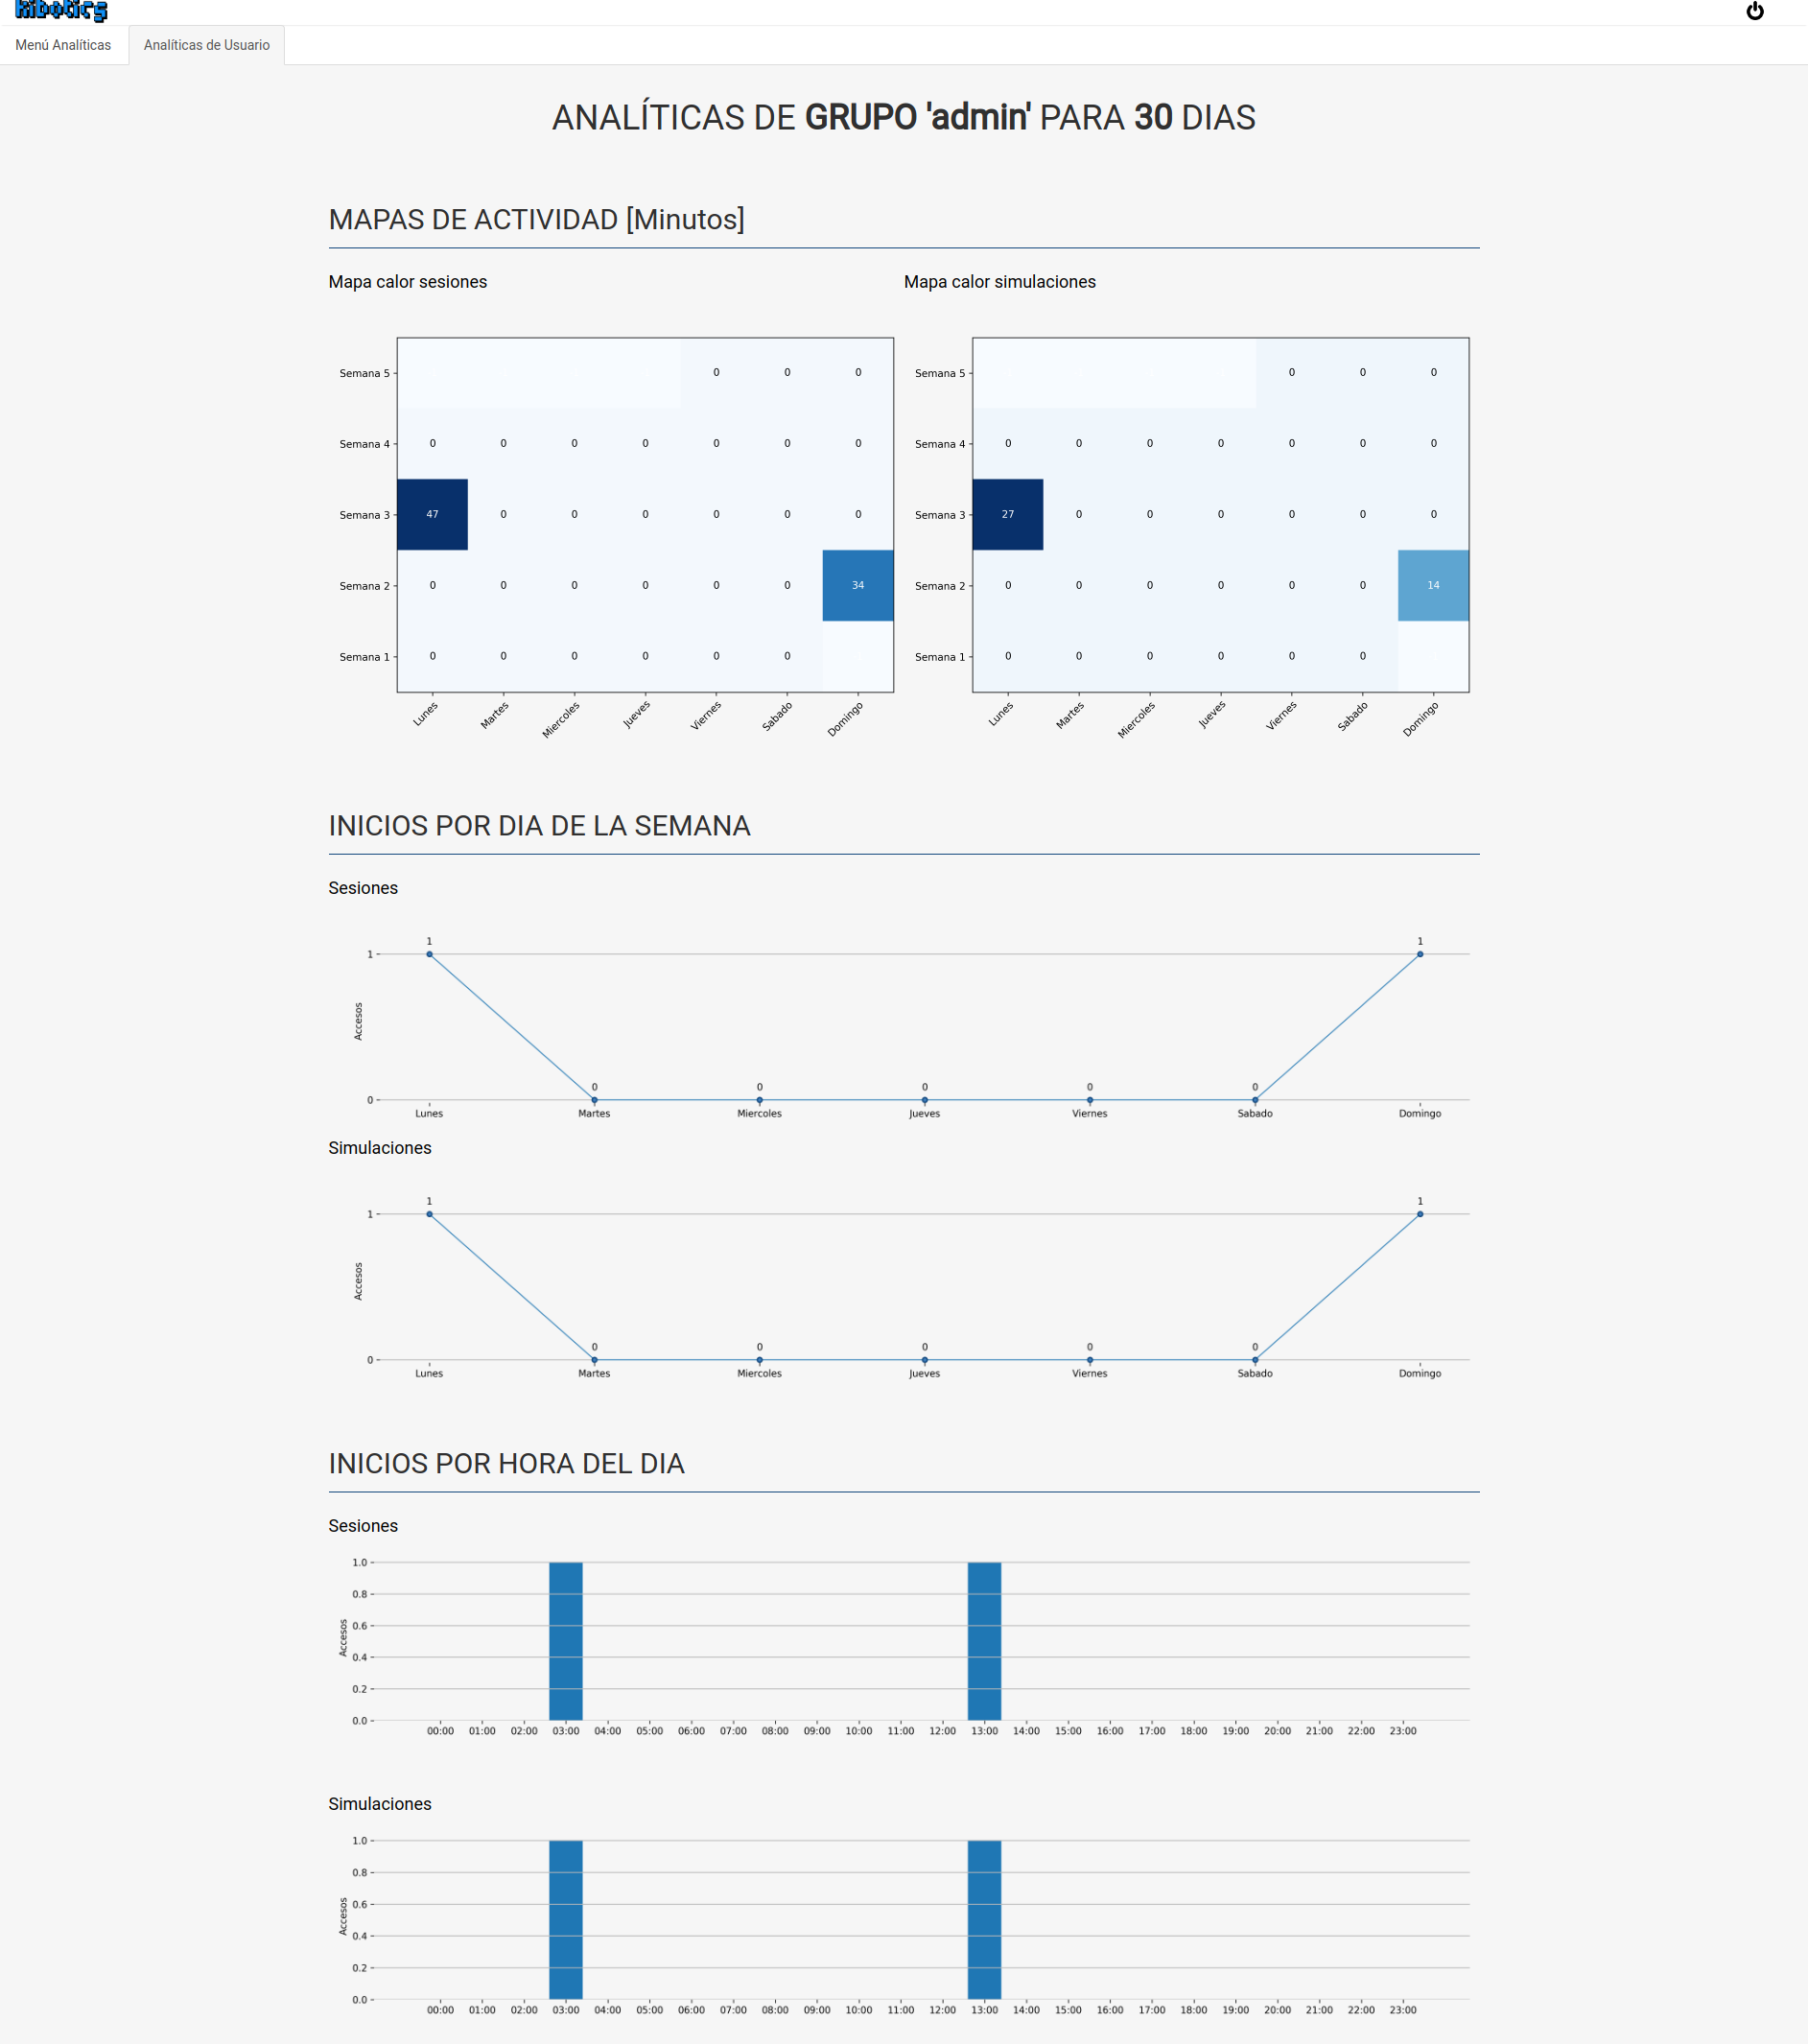
\includegraphics[width=17cm, keepaspectratio]{img/primer_prototipo_1.png}
			\caption{Analíticas del primer prototipo parte 1.}
			\label{fig:primer_prototipo_1}
		\end{figure}

		
		En la Figura \ref{fig:primer_prototipo_1}, se puede observar una primera parte con dos mapas de calor, los cuales representan la actividad semana a semana (filas) en el servidor web de Kibotics para los distintos eventos de sesión y simulación. El color será más intenso cuantos más sean los minutos invertidos en ese evento para cada uno de los días o celdas.\\
		
		En una segunda parte de esta misma figura se representan 4 visualizaciones más con los accesos a sesiones y simulaciones separadas en dos grupos. Una primera agrupación con los accesos por día de la semana, a continuación, el segundo grupo con accesos divididos por la hora del día a la que fueron realizadas.\\
		
		En la Figura \ref{fig:primer_prototipo_2} se representan las dos últimas secciones de este primer prototipo. Una primera sección con los tiempos totales y medios que el grupo de usuarios o usuario ha pasado en cada uno de los ejercicios a los que ha accedido. Finalmente, una última visualización que representa con un mapa geográfico la localización desde la que cada usuario ha accedido a la plataforma educativa.\\
		
		\begin{figure}[H]
			\centering
			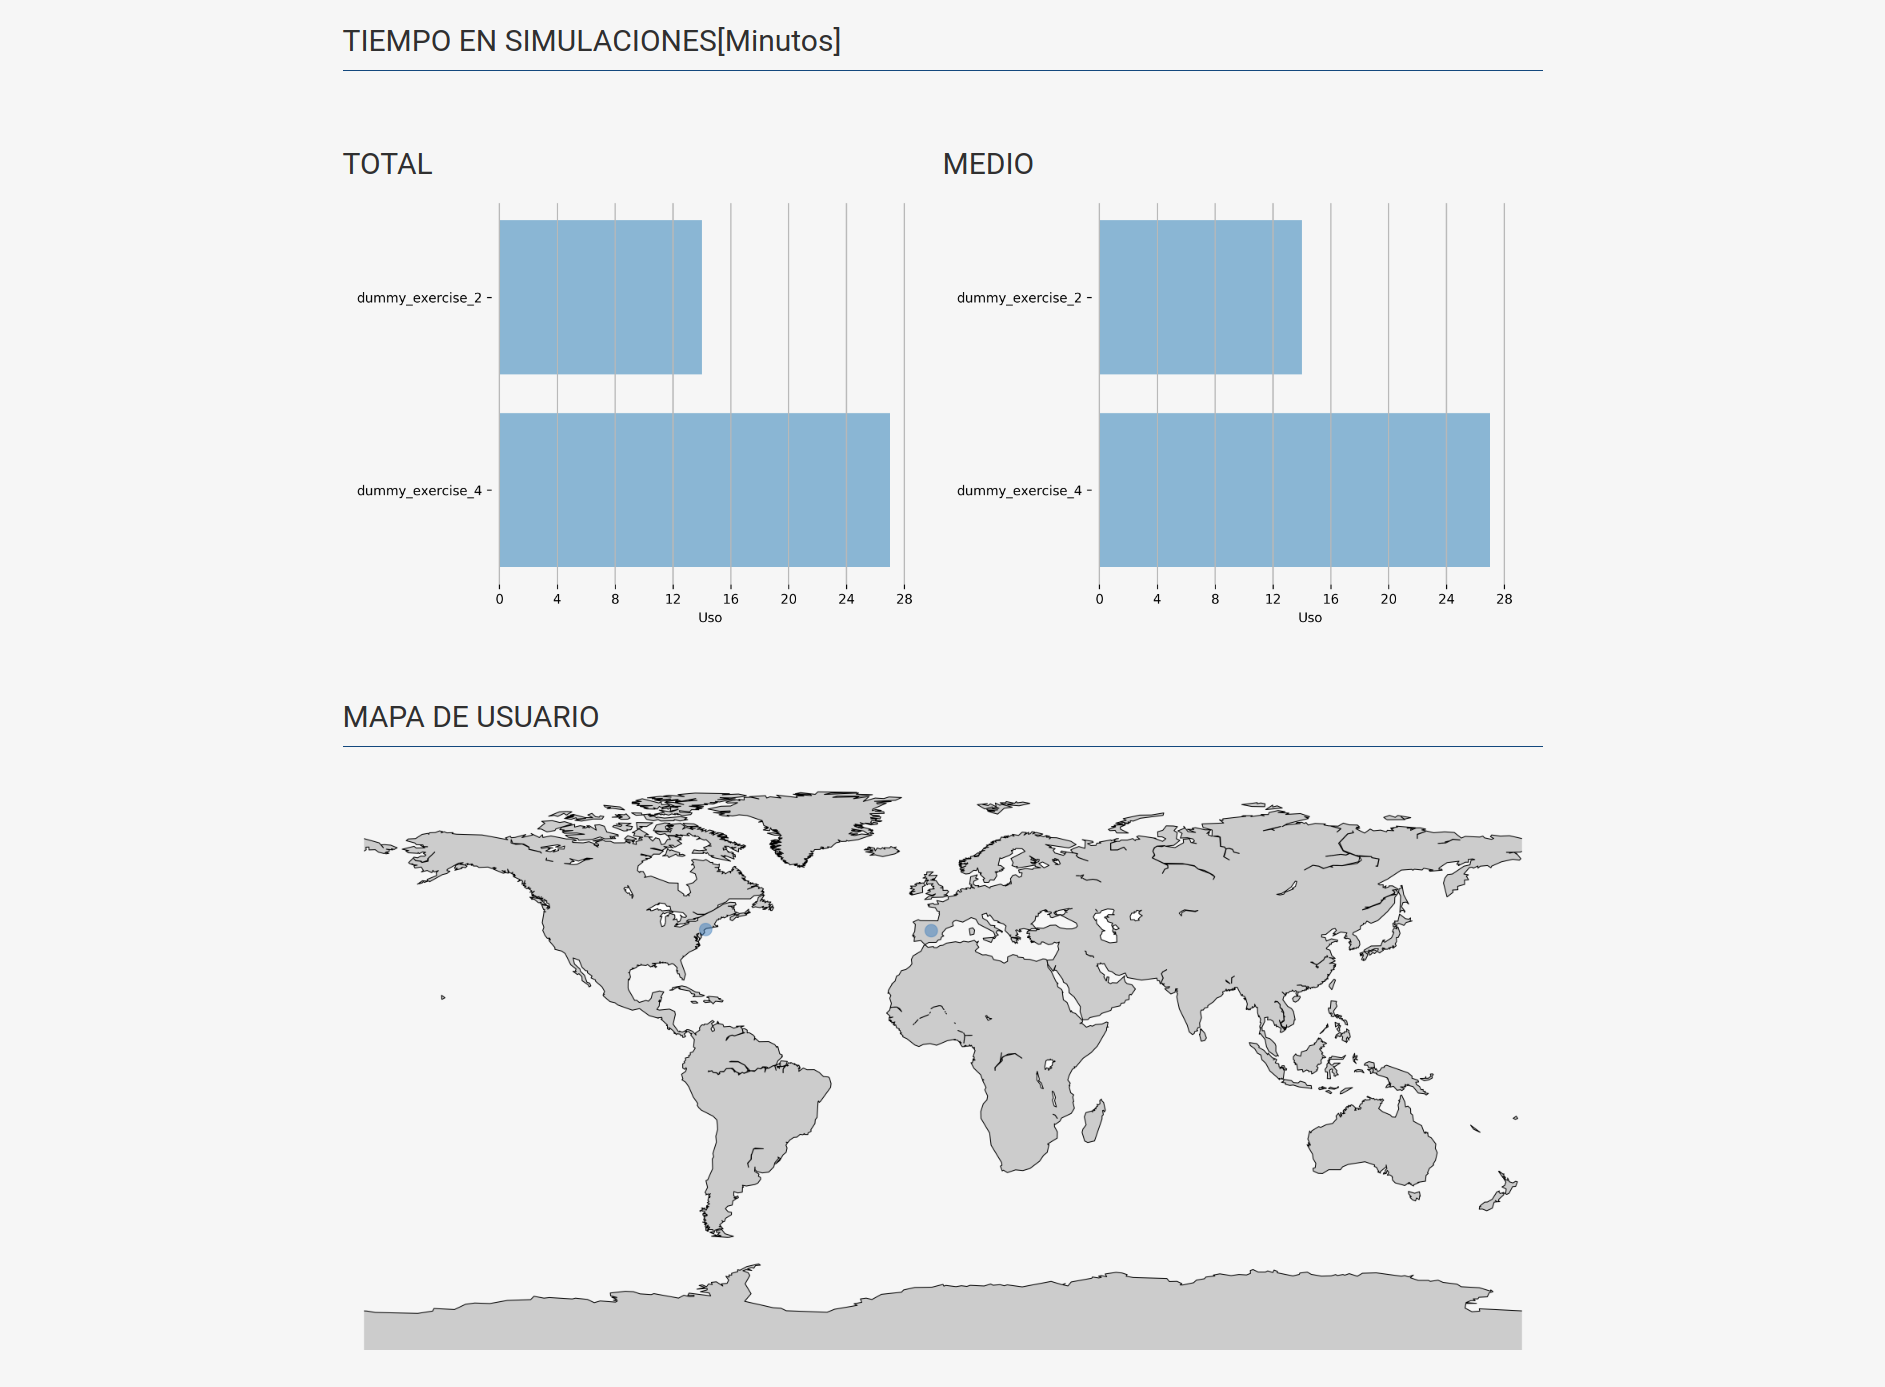
\includegraphics[width=17cm, keepaspectratio]{img/primer_prototipo_2.png}
			\caption{Analíticas del primer prototipo parte 2.}
			\label{fig:primer_prototipo_2}
		\end{figure}
		
		Este primer prototipo desarrollado de analíticas automáticas dentro de la plataforma Kibotics es bastante completo pero también tiene ciertos inconvenientes. Primero, falta cierta información útil que podría ser representada, como desde qué dispositivos acceden los usuarios o la actividad de los usuarios no registrados que simplemente visitan la web de la plataforma pero no llegan a registrarse o usarla.\\
		
		Las visualizaciones generadas, al estar insertadas como imágenes, carecen de interactividad, la cual sería muy útil para tener información extra o poder realizar filtrados más finos de los datos. Además, al tener que renderizar cada una de estas imágenes individualmente, tarda unos segundos en mostrar las visualizaciones.
	
	
	\cleardoublepage 
	\chapter{Analíticas basadas en Elasticsearch y Kibana} 
	\label{chap:segundo_prototipo} 
		En este capítulo se describen las nuevas tecnologías utilizadas en la versión final del módulo de analíticas que sustituyen a MongoDB y Matplotlib. Para enriquecer los datos que se estaban almacenando por las sondas del servidor, a esta nueva versión de la herramienta, se han añadido nuevas sondas y enriquecido las existentes. También se detallan la creación de recursos de prueba para que los futuros desarrolladores puedan integrar estas tecnologías en local.
	
	\section{Diseño} 
	\label{sec:2_diseno} 
%		cambiar cosas sobre la figura del cap 4
%		ahora ddbb elasticsearch xk
%		ahora se conecta a kibana para la visualizacion xk
%		descripciona panoramica
		Para el desarrollo de las mejoras necesarias de la herramienta de analíticas, el primer paso es realizar un diseño con los cambios a implementar así como las nuevas tecnologías involucradas. \\
		
		El primer prototipo  estaba basado en MongoDB como base de datos de logs, y con Matplotlib como generador de visualizaciones. Pese a ser bastante completo, carece de cierta información útil como datos de visitantes a la aplicación o acerca del \textit{software} y \textit{hardware} utilizado por los usuarios. Además, debido a la necesidad de renderizar cada una de las imágenes en Python, el subsistema de analíticas era lento. \\
		
		Es por esto, que se decide cambiar la tecnología de visualización de datos a Kibana. Al ser Kibana parte del stack ELK, la base de datos cambia a Elasticsearch para poder utilizar todo el potencial que este ecosistema ofrece. \\
		
		Para enriquecer los datos almacenados y evitar tener que cruzarlos como se detalla en la subsección \ref{subsec:matplotlib_kibotics}, se van a añadir más sondas de almacenamiento, esta vez con datos relativos a la actividad de los visitantes de la plataforma educativa. Además, se van a unificar las tablas en las que se almacenarán registros similares, evitando tener así que cruzar datos. Estos cambios reducirán el coste computacional de la herramienta haciéndola así más rápida. \\
		
		El nuevo diseño y los cambios de tecnología involucrados en este prototipo final se pueden ver representados de forma esquemática en la Figura \ref{fig:arquitectura_kibotics_2}. 
		
		\begin{figure}[H]
			\centering
			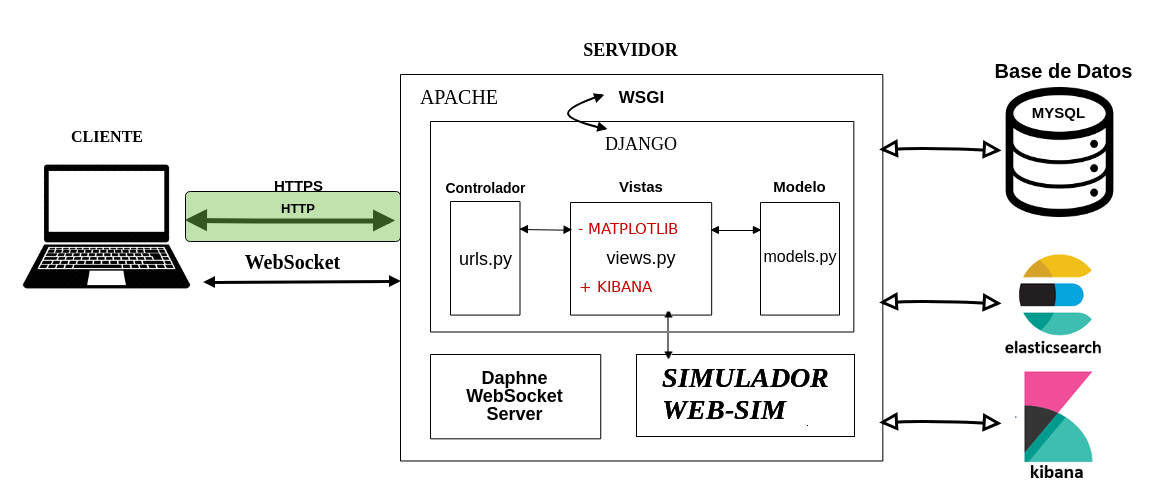
\includegraphics[width=16cm, keepaspectratio]{img/esquema_Kibotics_2.png}
			\caption{Arquitectura Kibotics segundo prototipo.}
			\label{fig:arquitectura_kibotics_2}
		\end{figure}
	
	\section{Implementación} 
	\label{sec:2_implementacion} 
	
		En esta sección se detallan los cambios involucrados en el desarrollo de la herramienta de analíticas para la integración de Elasticsearch como base de datos y Kibana como herramienta de visualización. Además, de esta versión final de la herramienta, se explica la generación de recursos de prueba para futuros desarrolladores de Kibotics.
	\subsection{Elasticsearch en Webserver}
	\label{subsec:elasticsearch_kibotics}
	
		El primer paso en el proceso de mejora de la herramienta es el cambio de base de datos. Para hacer uso del stack ELK, es necesario sustituir MongoDB por Elasticsearch. Para esto lo primero será instalar e iniciar un servicio de Elasticsearch en local \footnote{https://www.elastic.co/guide/en/elasticsearch/reference/current/targz.html}.\\
				
		Una vez iniciado el servicio Elasticsearch, ya dispondremos de la base de datos sobre la que guardar los registros de log o documentos, como se llaman en Elasticsearch. Similar a las tablas de las que hacía uso MongoDB, estos documentos se almacenan en índices, cada uno de los cuales está definido por un esquema de campos y tipologías que definen la estructura de los documentos que almacenan.\\
		
		Se podrán crear tantos índices como sea necesario, para consultarlos se puede lanzar una sentencia por terminal, o acceder con la IP y el puerto desde un navegador a la \texttt{API REST} configurada en instalación. Un ejemplo de llamada para un índice llamado index\_name\_test es la siguiente:
		
		{\footnotesize
		\begin{verbatim}
			http://127.0.0.1:9200/index_name_test/_search/?size=1000&pretty
		\end{verbatim}
		}
		
		El siguiente paso es la integración de Elasticsearch en Django. Se realizará haciendo uso de la librería Python \texttt{django\_elasticsearch\_dsl}. Para migrar de MongoDB a Elasticsearch se han realizado dos pasos: creación de los índices y migración de las sondas que almacenan los logs de MongoDB a Elasticsearch.\\
		
		
		El primer paso consistió en crear los índices de Elasticsearch. Estos índices son muy similares a los modelos que se utilizan en Django para representar la información de la base de datos. Para esta versión de la herramienta se crean los siguientes índices: 				
		
		\begin{itemize}
			\item \texttt{kibotics\_session\_log}: índice en el que se almacenan los eventos referentes a las sesiones.
			
			\item \texttt{kibotics\_simulation\_log}: índice en el que se almacena la información relativa a las simulaciones.
			
			\item \texttt{kibotics\_error\_log}: índice en el que se almacenan los eventos referentes a los errores.
			
			\item \texttt{kibotics\_visit\_log}: índice en el que se almacena la información relativa a las visitas.
		\end{itemize}				
		
		Para evitar la problemática que surgió durante el desarrollo del primer prototipo, relativo al cálculo de la duración de los eventos, se ha eliminado el campo que almacenaba la fecha. Para sustituirlo, se han añadido dos nuevos campos a los índices de Elasticsearch los cuales establecerán el inicio y fin de cada evento, unificando así los dos registros de log que se tenían en la primera versión.\\
		
		Por otro lado, el campo \texttt{USER\_AGENT}, que se almacenaba anteriormente y ofrecía información acerca del dispositivo y software que utilizaban los visitantes de la web, ha sido dividido y sustituido con la información del navegador, dispositivo y sistema operativo. Cada uno con su propio campo en los esquemas de los índices de Elasticsearch. Ofreciendo así la información de forma más clara y eliminando ciertos datos no útiles para las visualizaciones que se quieren generar.\\
		
		Para trabajar en Kibana con mapas geográficos es necesario guardar tanto la longitud como la latitud, para lo cual se hará uso de una tipología de campo ya existente en Elasticsearch llamado \textit{Geo Point} que almacenará en un diccionario ambas variables.\\
		
		Para complementar las nuevas sondas, que se han mencionado anteriormente y se explicarán con más detalle a continuación, es necesario la creación de un nuevo índice de visitas, en el que se registrarán los accesos a la pagina principal de la aplicación, estén o no registrados.\\
		
		Un ejemplo de la definición en Django del índices de sesiones de Kibotcis Webserver en el fichero \texttt{documents.py} es:
		
		{\footnotesize
		\begin{verbatim}
			from django_elasticsearch_dsl import Document, Text, Date, Double, GeoPoint, Ip
			
			class SessionDocument(Document):
			    username = Text()
			    start_date = Date()
			    end_date = Date()
			    duration = Double()
			    client_ip = Ip()
			    browser = Text()
			    os = Text()
			    device = Text()
			    location = GeoPoint()
			
			    class Index:
			        name = 'kibotics_session_log'
			        settings = {
			            'number_of_shards': 1,
			            'number_of_replicas': 0
			        }		
		\end{verbatim}
		}
		
		Con todo esto, se tiene una base sólida sobre la que almacenar la información de logs, solo falta modificar el guardado en Elasticsearch, migar las sondas que almacenan los registros de log.\\
		
		Para enriquecer las sondas ya existentes y hacer uso de los nuevos campos e índices creados, se han añadido nuevas sondas para almacenar eventos de visitantes, así como sondas para optimizar la monitorización de salida de sesiones y simulaciones y evitar no tener un registro de inicio sin su correspondiente registro de fin de evento por un cierre busco de la aplicación o inactividad.\\
		
		Las sondas de inicio de los eventos son similares a las que se tenían anteriormente en MongoDB, un ejemplo para la sonda de inicio de simulación es:
		
		{\footnotesize
		\begin{verbatim}
			SimulationDocument(
			    username = "USERNAME_TEST",
			    start_date = start_date_object_test,
			    end_date = start_date_object_test,
			    duration = 0.0,
			    client_ip = "CLIENT_IP_TEST",
			    simulation_type = "SIMULATION_TYPE_TEST",
			    exercise_id = "EXERCISE_ID_TEST",
			    browser = "BROWSER_TEST",
			    os = "OS_TEST",
			    device = "DEVICE_TEST",
			    location = {'lat': latitude_double_test, 'lon': longitude_double_test}
			).save()
		\end{verbatim}
		}
	
		Sin embargo, al unificar los registros de entrada y salida en un único documento las sondas de fin de sesión/simulación cambian. Tendrán que buscar en Elasticsearch el último documento no finalizado en el índice para el usuario del cual se quiera cerrar el evento y sustituir tanto los campos \texttt{end\_date} como \texttt{duration}. \\
		
		Esto se realiza gracias al identificador que cada documento indexado posee al cual se le realiza una operación \textit{update} con los nuevos campos. Un ejemplo de cierre de sesión en Python es:
		
		
		{\footnotesize
		\begin{verbatim}
			# Búsqueda del ultimo registro de sesión no cerrado
			latest_session = Search(index="kibotics_session_log*") \
			                .query("match", username=username) \
			                .query('match', duration=0) \
			                .sort({"start_date": {'order': 'desc'}})[0]
			
			# Actualización de los campos end_date y duration
			for hit in latest_session:
			    duration = datetime.now() - datetime.strptime( \
			    hit.start_date, \
			    "%Y-%m-%dT%H:%M:%S.%f")
			
			    Elasticsearch(settings.ELASTICSEARCH_DSL['default']['hosts']) \
			        .update(index = 'kibotics_session_log', 
			                id = hit.meta.id,
			                body = {"doc": {
			                            'end_date' : datetime.now(), 
			                            'duration' : duration.total_seconds()
			                            }
			                        })
		\end{verbatim}
		}
	
		Durante el desarrollo de está lógica es útil hacer uso de la interfaz de Elasticsearch para comprobar que todos estos campos están siendo creados y actualizados correctamente. A esta interfaz se accede mediante la \texttt{URL} y puerto configurados durante el proceso de instalación.\\
		
		En esta \texttt{API}, podremos realizar filtrados por campos e índices haciendo uso de expresiones regulares \textit{Regex}, por ejemplo para acceder al índice en el que se almacenan los documentos relativos a los logs de sesiones, podremos acceder mediante la siguiente \texttt{URL}:
		
		{\footnotesize
		\begin{verbatim}
			http://127.0.0.1:9200/kibotics_session_log/_search/?size=1000&pretty
		\end{verbatim}
		}
	
		En la Figura \ref{fig:api_elasticsearch} se puede observar la respuesta que se obtiene de la API de Elasticsearch en el navegador a la llamada anterior.
		
		\begin{figure}[H]
			\centering
			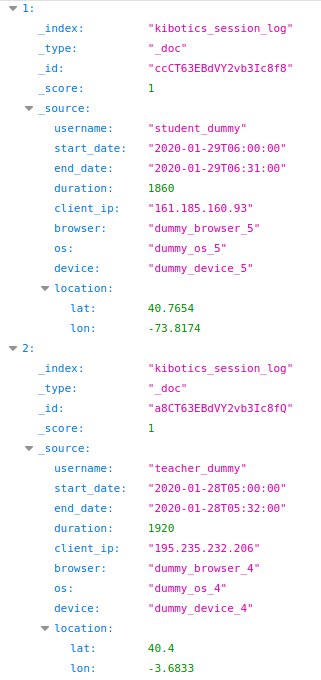
\includegraphics[width=6cm, keepaspectratio]{img/api_elasticsearch.png}
			\caption{API Rest Elasticsearch.}
			\label{fig:api_elasticsearch}
		\end{figure}
		
	
	\subsection{Kibana en Webserver}
	\label{subsec:kibana_kibotics}
		Para acceder a Kibana, deberemos primero instalar y ejecutar el servicio\footnote{https://www.elastic.co/guide/en/kibana/current/targz.html}. Una vez Kibana está ejecutando podremos acceder a su interfaz gráfica mediante la URL y puerto configurado en la instalación:
		
		{\footnotesize
		\begin{verbatim}
			http://127.0.0.1:5601/app/kibana#/home
		\end{verbatim}
		}
	
		Ya con datos en Elasticsearch almacenados y como se muestra en la Figura \ref{fig:index_pattern_kibana}, Kibana nos pedirá que añadamos los índices sobre los que queremos obtener soporte y seleccionemos el campo sobre el que se filtrarán temporalmente estos logs. En este caso se utilizará el campo start\_date.
		
		\begin{figure}[H]
			\centering
			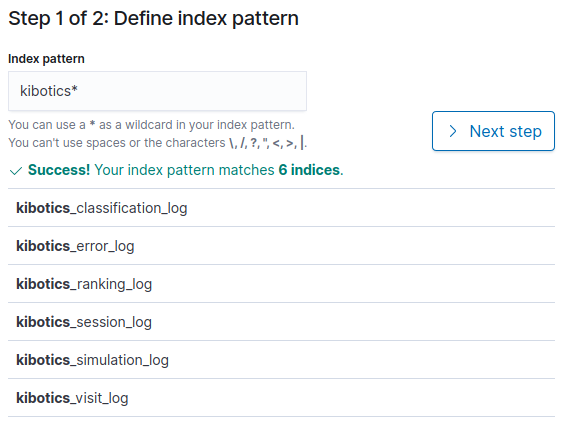
\includegraphics[width=11cm, keepaspectratio]{img/index_pattern_kibana.png}
			\caption{Creación de índices en Kibana.}
			\label{fig:index_pattern_kibana}
		\end{figure}
		
		Configurados todos los índices en Kibana se tiene una primera visualización de los documentos indexados en Elasticsearch en la pestaña \textit{Discover} de Kibana. En esta pestaña podremos ver todos los logs que estén almacenados en los índices, así como un histograma en el que se podrá ver gráficamente la evolución de estos índices en el tiempo. Además, esta sección \textit{Discover} proporciona la posibilidad de filtrar por rangos de fechas y campos así como se tenía en el primer prototipo de este proyecto.\\
		
		Esta sección ya nos da una primera pincelada de la potencia de procesamiento de Kibana, así como la sencillez de implementación y despliegue. Las consultas son instantáneas, notablemente más rápidas que las realizadas en el primer prototipo desarrollado.\\
		
		\begin{figure}[H]
			\centering
			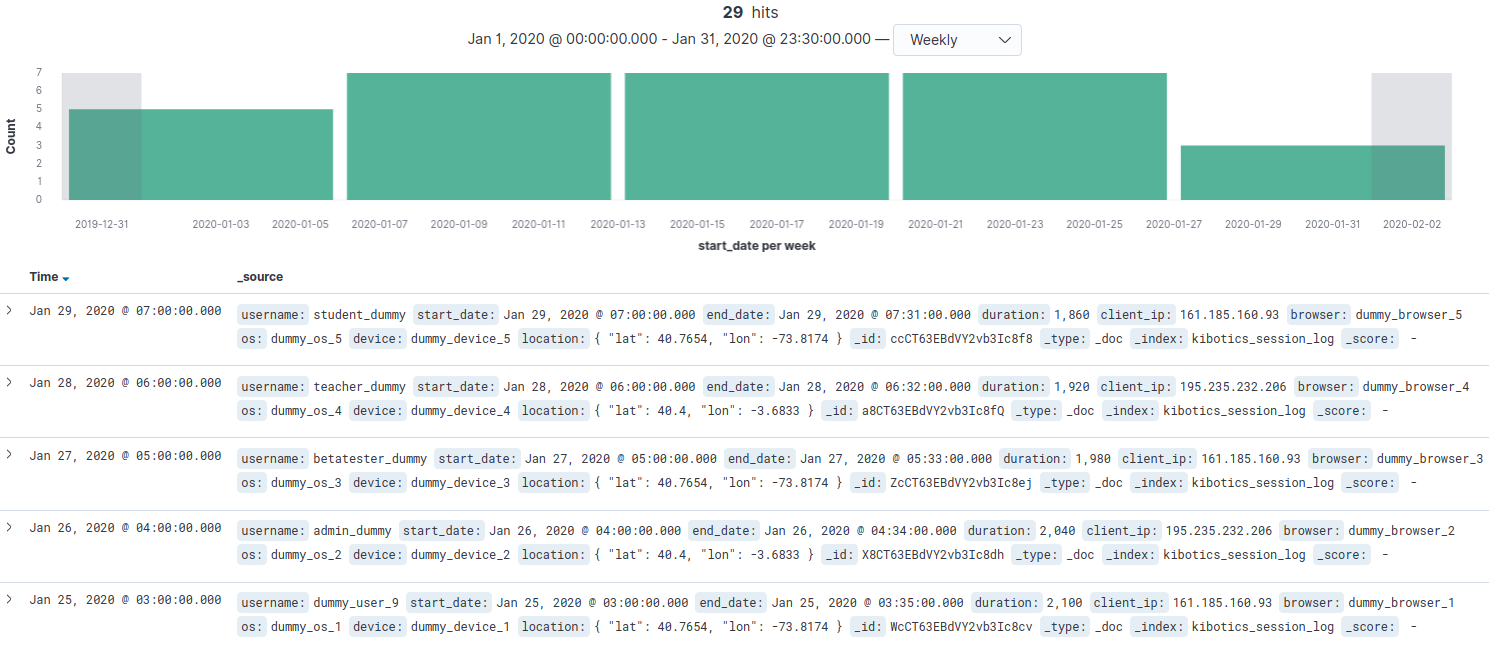
\includegraphics[width=15cm, keepaspectratio]{img/discover_kibana.png}
			\caption{Sección \textit{Discover} en Kibana.}
			\label{fig:discover_kibana}
		\end{figure}
		
		Kibana ofrece la posibilidad de creación de \textit{scripted fields}, campos cuyo valor deriva de otros campos o datos ya indexados. Generados en un lenguaje muy similar a \texttt{C} llamado \texttt{painless}. \\
		
		Para el módulo de analíticas que se quiere desarrollar, y en especial para las visualizaciones que filtran por día de la semana y por hora del día, se han creado dos \textit{scripted fields} para cada uno de los índices utilizados. Estos son \texttt{day\_of\_week} y \texttt{hour\_of\_day}, el código painless utilizado para la creación de estos campos es el siguiente:
		
		{\footnotesize
		\begin{verbatim}
			// day_of_week
			["", "1 Lunes", "2 Martes", "3 Miercoles", "4 Jueves", "5 Viernes",
			"6 Sabado", "7 Domingo"] [doc['start_date'].value.dayOfWeek]
			
			// hour_of_day
			doc['start_date'].value.hourOfDay
		\end{verbatim}
		}
	
		Con estos \textit{scripted fields} además de los campos ya almacenados en los documentos, Kibana dispone de todos los datos necesarios para la creación de las visualizaciones. Para ello, en la sección \textit{Visualize}, Kibana tiene una colección de distintas plantillas gráficas. Estas plantillas serán las que se configuren con los índices, documentos y campos a usar para la generación de los distintos tipos de visualizaciones. En la Figura \ref{fig:visualization_selector} se muestran algunas de las visualizaciones que Kibana ofrece.
		
		\begin{figure}[H]
			\centering
			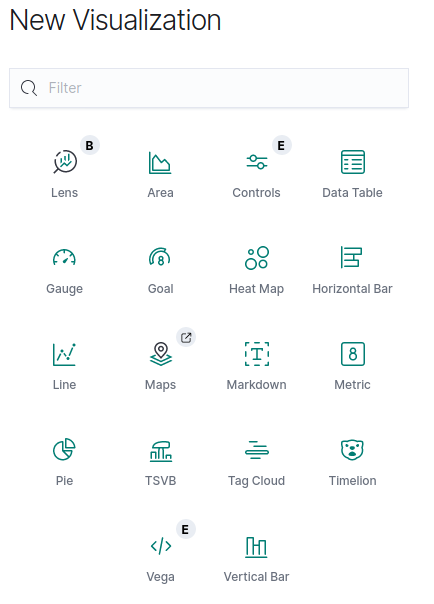
\includegraphics[width=5cm, keepaspectratio]{img/visualization_selector.png}
			\caption{Menú creación de visualizaciones.}
			\label{fig:visualization_selector}
		\end{figure}
		

		Ya creadas las visualizaciones, solo quedará integrarlas en Kibotics sustituyendo las generadas en Matplotlib. Para ello se creará una vista \texttt{menú} con la que se seleccionará a que tipo de analíticas se quiere acceder. Este menú selector de analíticas es el mostrado a continuación en la Figura \ref{fig:kibotics_analytics_menu}.
	
		\begin{figure}[H]
			\centering
			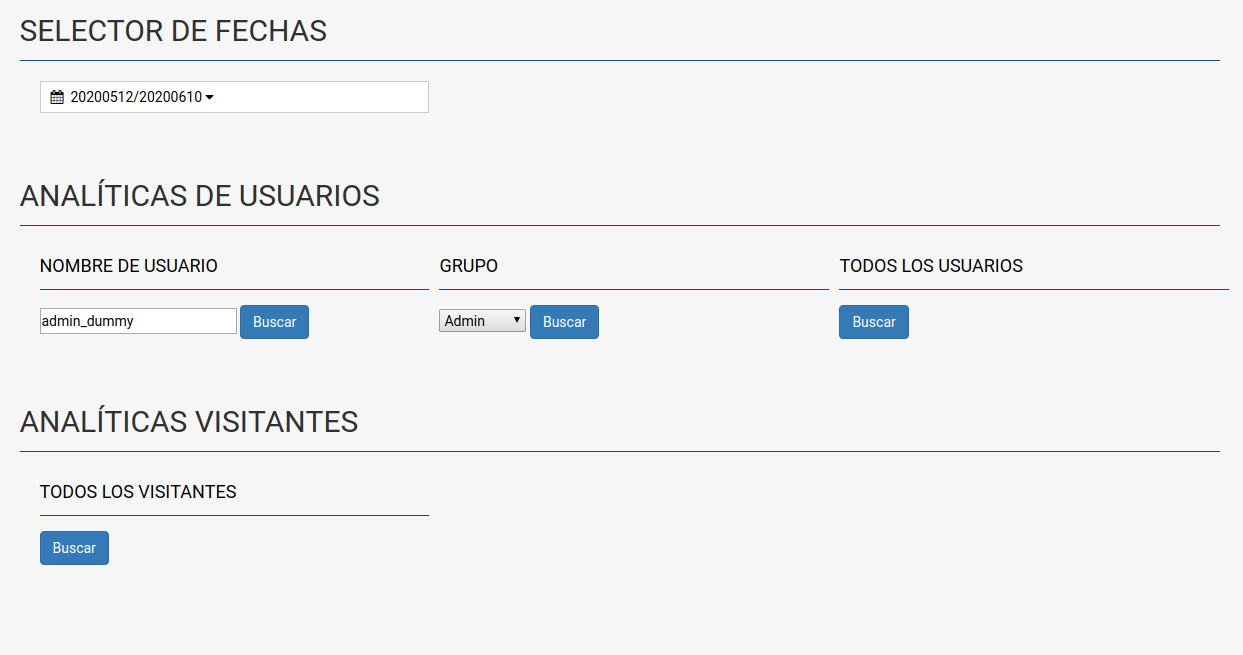
\includegraphics[width=14cm, keepaspectratio]{img/kibotics_analytics_menu.png}
			\caption{Menú de selección de analíticas en Kibotics}
			\label{fig:kibotics_analytics_menu}
		\end{figure}
		
		En esta vista se filtrará tanto por usuarios y grupos, como por fechas de las cuales se quieren analíticas. Una vez filtrado, Django generará automáticamente una \texttt{URL} con los datos seleccionados en el Menú de Kibotics. Esta \texttt{URL} dinámica apuntará a las visualizaciones de nuestro servicio de Kibana y será devuelta por el contexto de Django hasta las plantillas Django que lo insertarán en un elemento \texttt{HTML iFrame}.
	

	\section{Validación experimental} 
	\label{sec:2_validacion_experimental} 
%		video ilustrativo - pantallazos
%		creacion de base de datos dummy ES
%		creacion de base de datos dummy Kibana	


		Para esta versión final del módulo de analíticas, se han creado una amplia selección de visualizaciones de las que obtener información de actividad de los usuarios. Divididas en dos \textit{Dashboards} o tableros, el primero reservado a los visitantes no registrados y el segundo para analíticas de sesiones y simulaciones de usuarios registrados. A continuación, se mostrarán las visualizaciones creadas así como una explicación de lo que representan.\\
		
		Para tener un control del número de accesos a lo largo del tiempo se creó el histograma representado en la Figura \ref{fig:kibana_histogram}. Este histograma muestra los eventos almacenados en el índice \texttt{kibotics\_session\_log} dividido día a día en el eje de abscisas.	
		\begin{figure}[H]
			\centering
			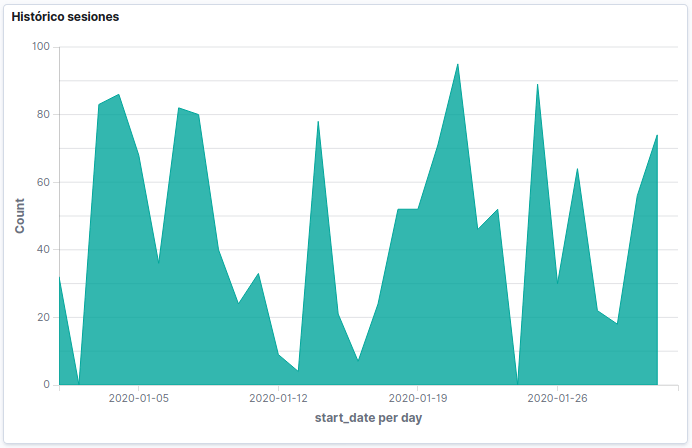
\includegraphics[width=9cm, keepaspectratio]{img/kibana_01_histogram}
			\caption{Histograma}
			\label{fig:kibana_histogram}
		\end{figure}
		
		Se ha creado un mapa de calor, que al igual que el histograma antes mencionado, representa la actividad de inicio de eventos. Dividido en columnas, cada una representa una semana con sus 7 días correspondientes. Un color más oscuro en la celda indica mayor actividad para ese día. Como se puede observar en la Figura \ref{fig:kibana_heatmap}, hay una visualización para las sesiones y otro para las simulaciones, división recurrente que se observa en distintas secciones del módulo Kibana desarrollado.
		\begin{figure}[H]
			\centering
			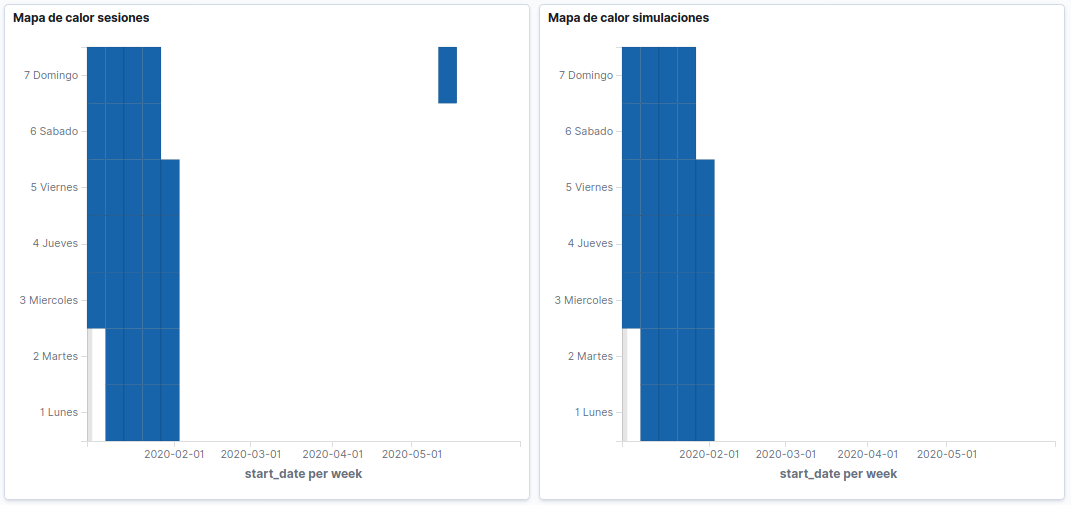
\includegraphics[width=13cm, keepaspectratio]{img/kibana_02_heatMap}
			\caption{Mapa de calor sesiones y simulaciones}
			\label{fig:kibana_heatmap}
		\end{figure}
		
		La Figura \ref{fig:kibana_dayofweek}, dividida en dos visualizaciones, representa la actividad tanto de sesiones como de simulaciones almacenada en los índices de Elasticsearch \texttt{kibotics\_session\_log} y \texttt{kibotics\_simulation\_log} respectivamente. En formato gráfico de barras vertical, los datos, filtrados por el día de la semana en que se registraron en el campo inicio de evento \texttt{start\_date}. \\
		
		\begin{figure}[H]
			\centering
			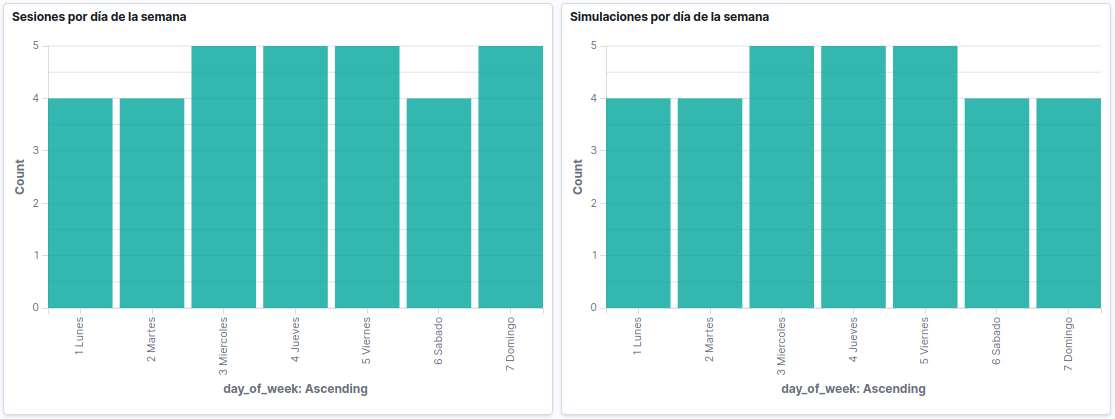
\includegraphics[width=14cm, keepaspectratio]{img/kibana_03_day_of_week}
			\caption{Gráfico de barras por día de la semana}
			\label{fig:kibana_dayofweek}
		\end{figure}
		
		La Figura \ref{fig:kibana_hourofday} muestra, en dos visualizaciones con gráficas de barras verticales, la actividad en el servicio web Kibotics. Filtrados, esta vez, por la hora del día en que se registraron los eventos. Como se puede observar, cada una de estas visualizaciones corresponde a uno de los eventos que han sido logueados en Elasticsearch y almacenados en los índices \texttt{kibotics\_session\_log} y \texttt{kibotics\_simulation\_log}.\\
		
		\begin{figure}[H]
			\centering
			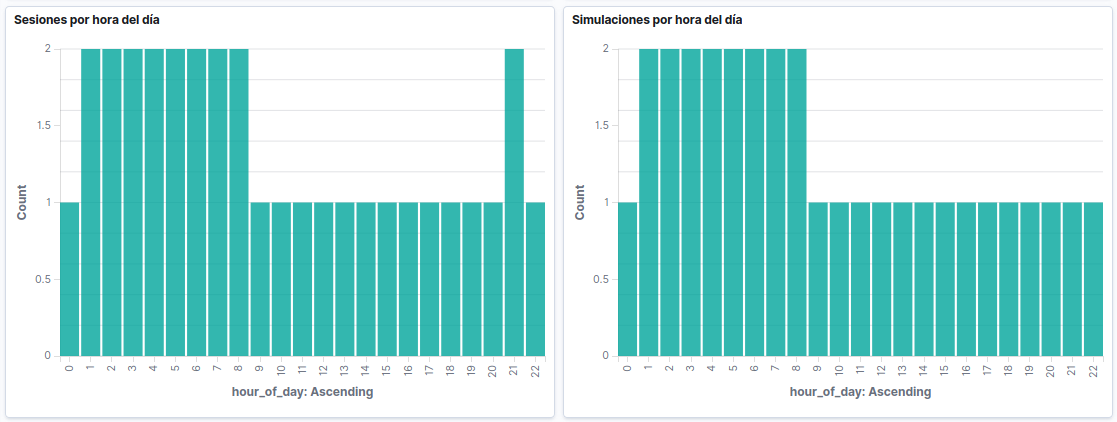
\includegraphics[width=14cm, keepaspectratio]{img/kibana_04_hour_of_day}
			\caption{Gráfico de barras por hora del día}
			\label{fig:kibana_hourofday}
		\end{figure}
		
		Para mostrar la actividad en las simulaciones que Kibotics ofrece, se han desarrollado las visualizaciones representadas en la Figura \ref{fig:kibana_simulations}. Dividido en dos gráficas de barras que representan el tiempo invertido por los usuarios. Esta información está almacenada en el campo \texttt{duration} del índice \texttt{kibotics\_simulation\_log}. La primera visualización muestra el tiempo total invertido y la última representa el tiempo medio invertido. \\
		\begin{figure}[H]
			\centering
			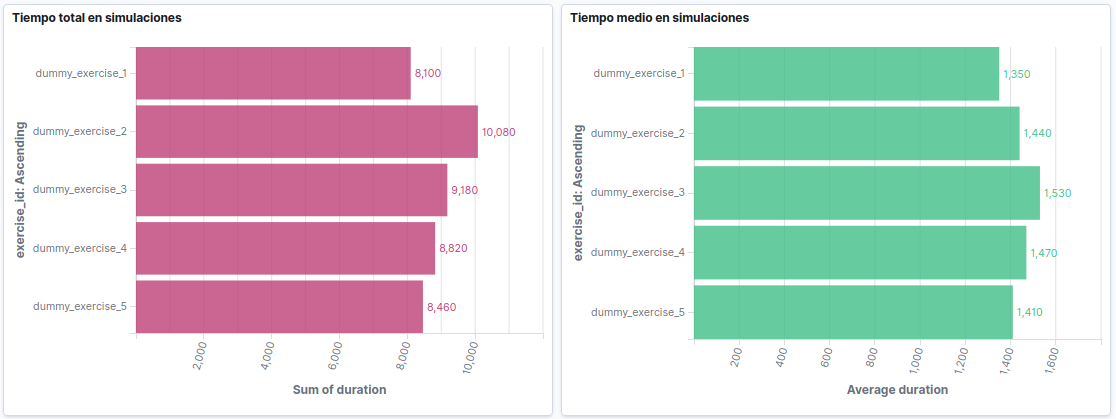
\includegraphics[width=13cm, keepaspectratio]{img/kibana_05_simulations}
			\caption{Gráfico de barras para tiempo total y medio en simulaciones}
			\label{fig:kibana_simulations}
		\end{figure}
		
		En la Figura \ref{fig:kibana_map}, se representa gráficamente la superficie terrestre, en ella se muestran eventos de inicio de sesión ocurridos para el rango de fechas seleccionado. Hace uso de los datos de latitud y longitud almacenados en formato \texttt{Geo Point} del índice \texttt{kibotics\_session\_log}.
		\begin{figure}[H]
			\centering
			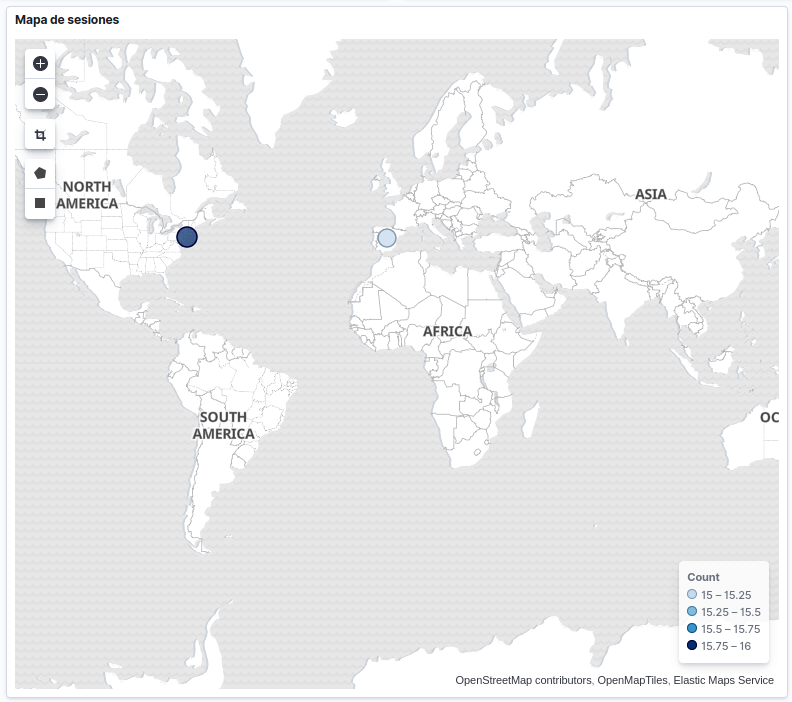
\includegraphics[width=11cm, keepaspectratio]{img/kibana_06_map}
			\caption{Mapa geográfico de sesiones}
			\label{fig:kibana_map}
		\end{figure}
		
		Para monitorizar el \textit{hardware} y \textit{software} utilizado por los usuarios de la web, se han desarrollado las tres gráficas circulares mostradas a continuación en la figura \ref{fig:kibana_pie}. Cada una de ellas representa porcentualmente campos almacenados en el índice de sesiones  \texttt{kibotics\_session\_log} que proporcionan información acerca del sistema operativo, dispositivo y navegador utilizados.
		\begin{figure}[H]
			\centering
			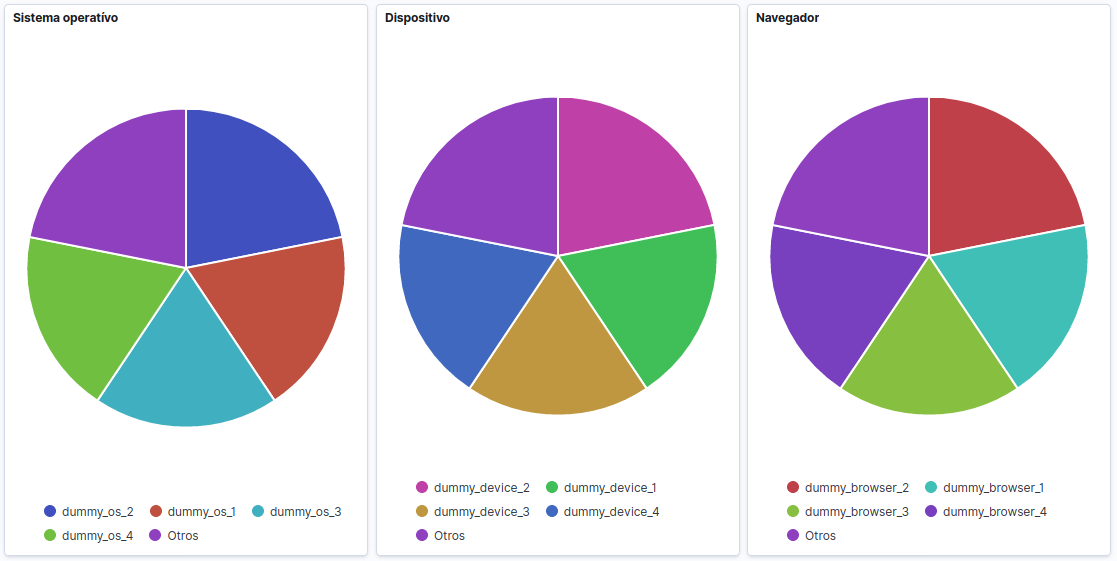
\includegraphics[width=14cm, keepaspectratio]{img/kibana_07_pie}
			\caption{Gráficas circulares para SO, Dispositivo y Navegador}
			\label{fig:kibana_pie}
		\end{figure}
		
		En la figura \ref{fig:kibana_latestevent}, se muestra una última sección con dos tablas de datos con los últimos eventos de sesión y simulación almacenados en los índices \texttt{kibotics\_session\_log} y \texttt{kibotics\_simulation\_log} de Elasticsearch para cada uno de los usuarios filtrados. 
		\begin{figure}[H]
			\centering
			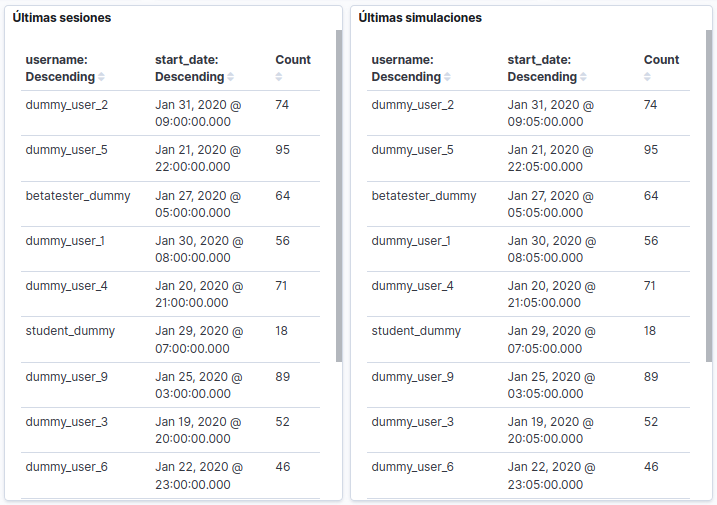
\includegraphics[width=12cm, keepaspectratio]{img/kibana_08_latest_event}
			\caption{Últimos eventos logueados}
			\label{fig:kibana_latestevent}
		\end{figure}
		
		Todas estas visualizaciones son interactivas y se puede filtrar por sus campos simplemente pulsando sobre ellas. Funcionalidad muy útil que no poseían las imágenes renderizadas que se generaban en el primer prototipo. Además, cada una de las visualizaciones del módulo desarrollado tiene una opción para ver los datos representados en texto plano e incluso descargarlos en formato \texttt{CSV} para su posterior tratamiento.\\
		
		Se han mostrado las visualizaciones referentes a la sección de sesiones y simulaciones de usuarios registrados ya que es la que más información proporciona, pero hay otra sección de analíticas de visitantes con unas visualizaciones de monitorización similares a las mostradas anteriormente.
		
	 	A continuación, en las siguientes figuras, se muestra Kibana ya integrado en la nueva vista de analíticas del servicio web Kibotics haciendo uso del \texttt{iFrame}.
				
		\begin{figure}[H]
			\centering
			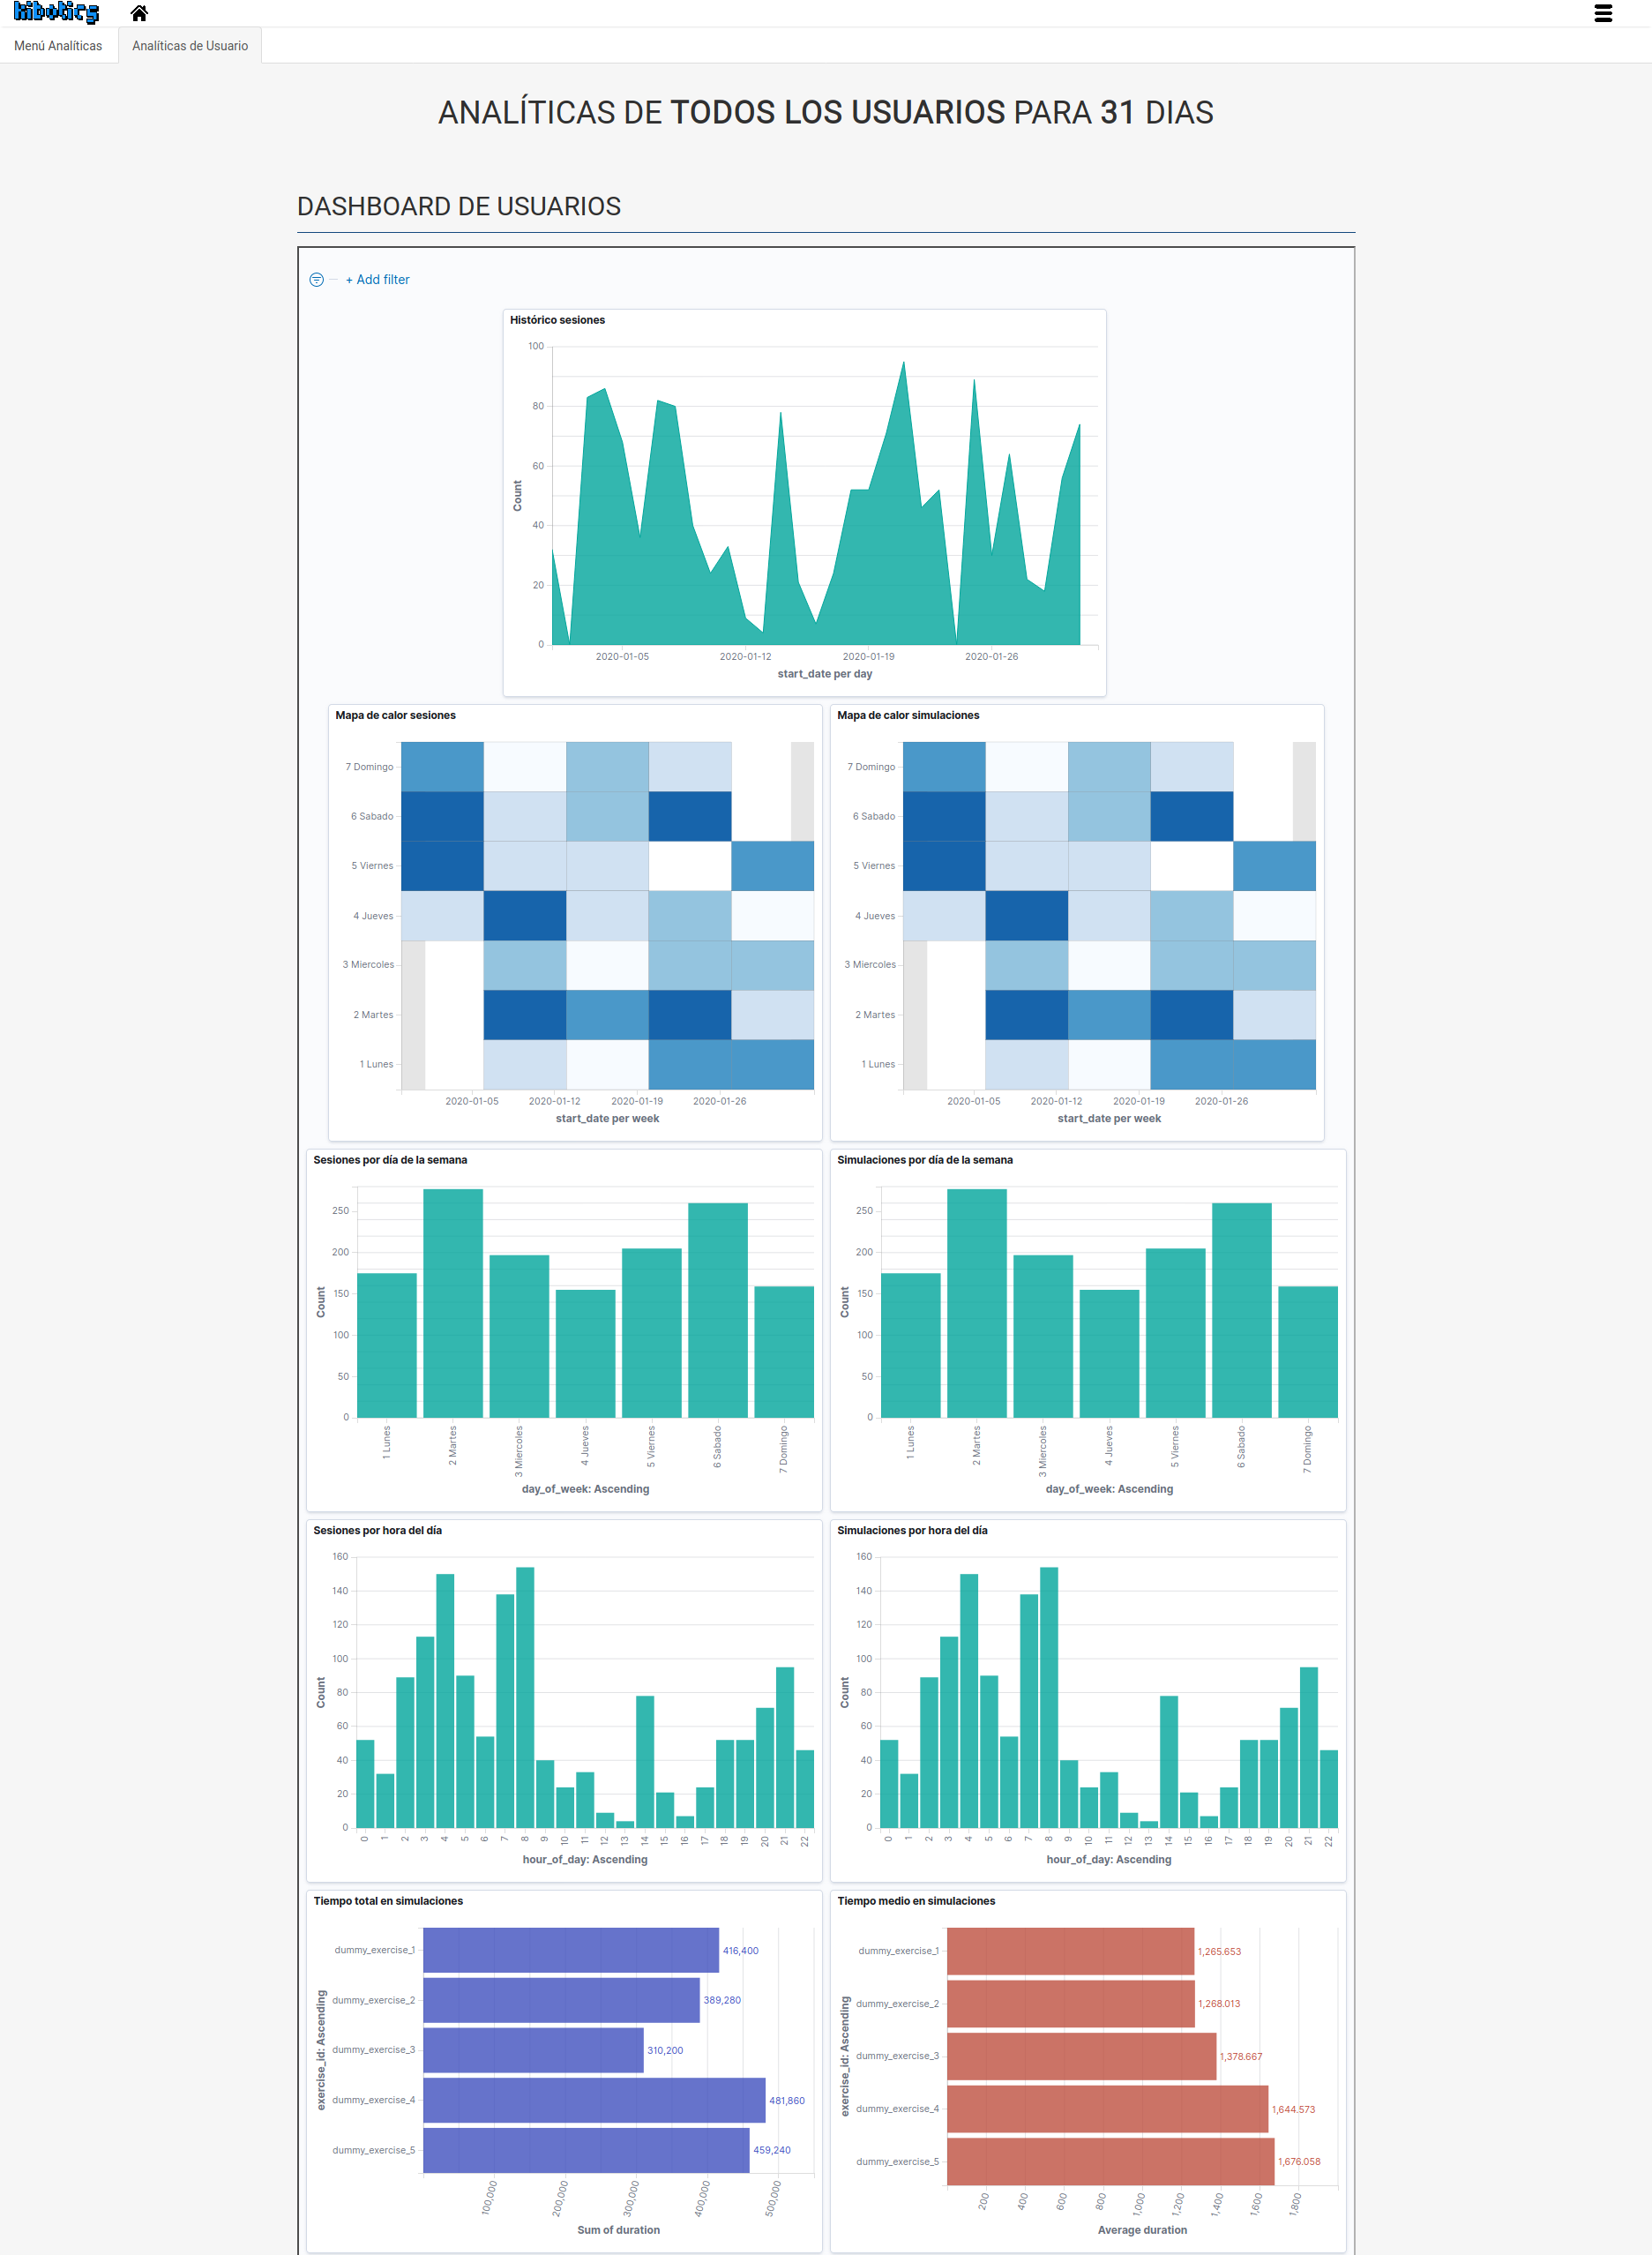
\includegraphics[width=15cm, keepaspectratio]{img/kibana_kibotics_01.png}
			\caption{Kibana en Kibotics parte 1}
			\label{fig:kibana_kibotics_01}
		\end{figure}
		\begin{figure}[H]
			\centering
			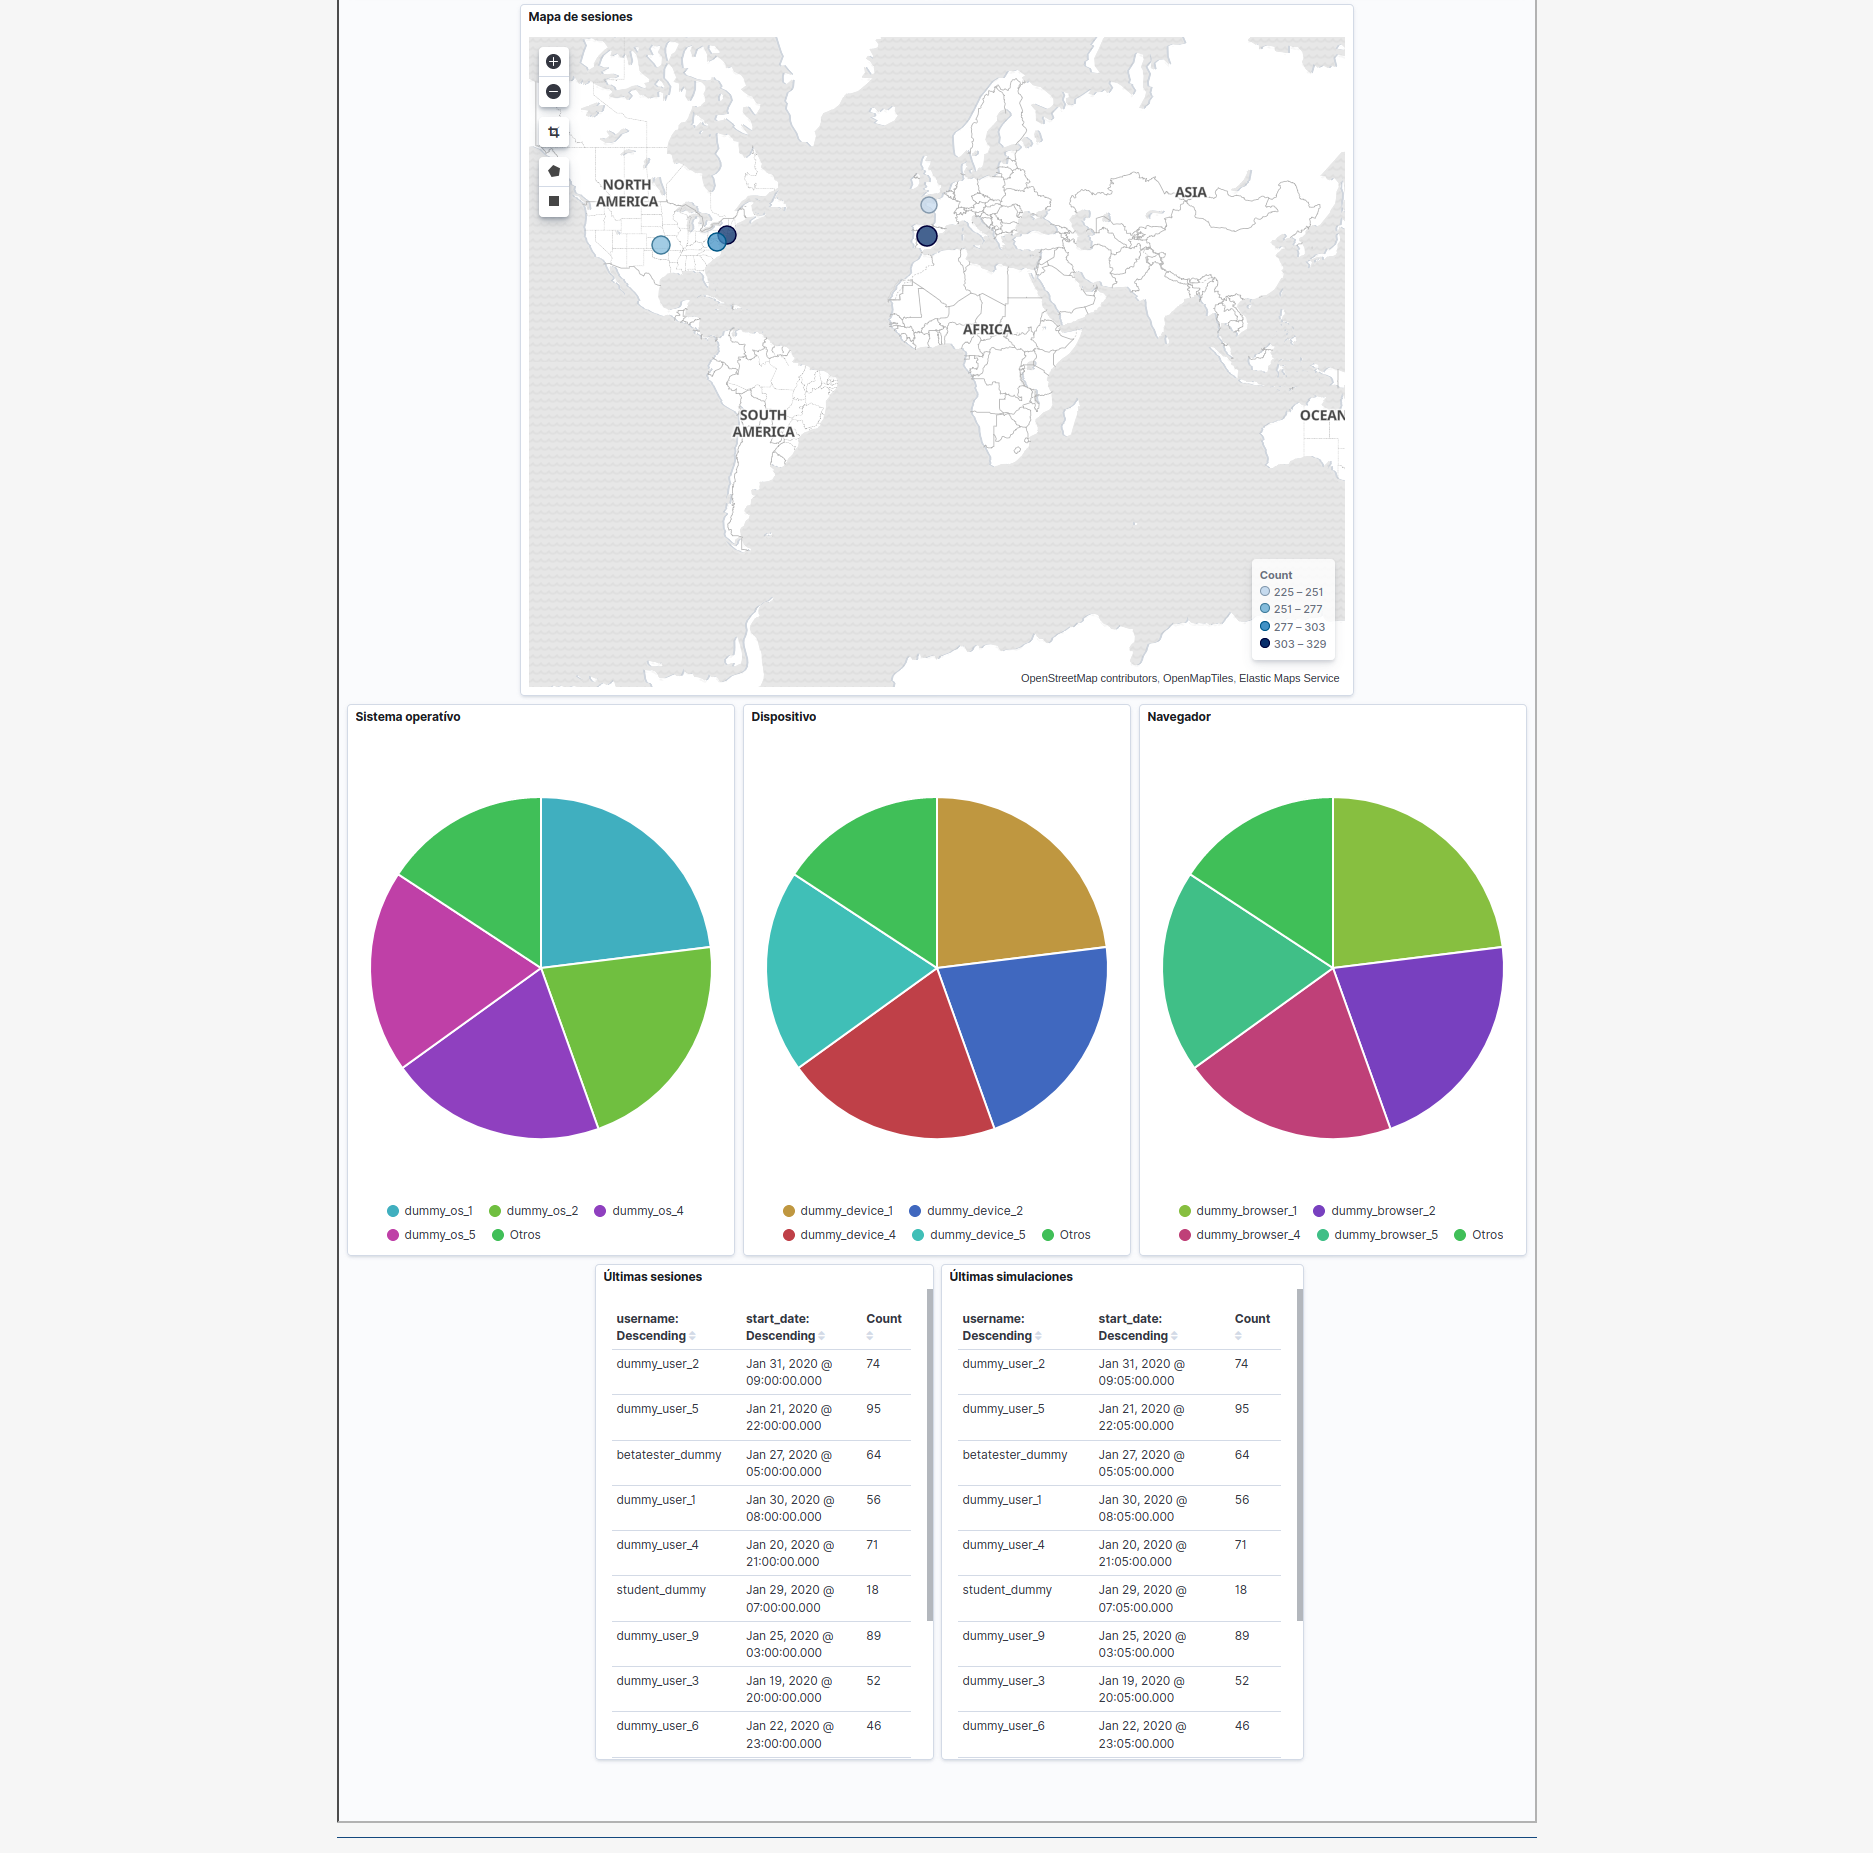
\includegraphics[width=15cm, keepaspectratio]{img/kibana_kibotics_02.png}
			\caption{Kibana en Kibotics parte 2}
			\label{fig:kibana_kibotics_02}
		\end{figure}
		

		Para proporcionar a los futuros desarrolladores los recursos necesarios con los que poder empezar a trabajar sin tener que crearlos de manera manual, se ha creado una base de datos dummy la cual ofrece una variedad de datos para todos los índices utilizados tanto en este proyecto, como en otros desarrollos paralelos.\\

		La creación de esta base de datos de pruebas se generó mediante un \textit{script} de Python que crea los índices y su estructura haciendo uso de la librería que Elasticsearch proporciona para Python.\\
		
		El \textit{script} creará todos los índices con sus respectivas estructuras y tipologías de datos. Un ejemplo para el índice de sesiones es:
		
		{\footnotesize
		\begin{verbatim}
			# Import librería Elasticsearch y conexión
			from elasticsearch import Elasticsearch
			client = Elasticsearch()
			
			# JSON con la estructura del índice
			session_mapping = {
			    "settings": {
			        "number_of_shards": 1,
			        "number_of_replicas": 0 },
			    "mappings": {
			        "properties": {
			            "username": { "type":"keyword" },
			            "start_date":{ "type":"date" },
			            "end_date":{ "type":"date" },
			            "duration": { "type":"double" },
			            "client_ip":{ "type":"ip" },
			            "browser": { "type":"keyword" },
			            "device":{ "type":"keyword" },
			            "location": { "type": "geo_point" },
			            "os":{ "type":"keyword" }
			        }
			    }
			}
			
			# Creación del índice en Elasticsearch
			client.indices.create( index="kibotics_session_log",
			                       body=session_mapping,
			                       ignore=400 )
		\end{verbatim}
		}
	
		Una vez creadas las estructuras de los índices, el siguiente paso es guardar todos los objetos con la información de prueba que se deseé guardar.\\
		
		Finalizada la ejecución del \textit{script} ya tendríamos los datos en nuestro servicio local de Elasticsearch. Para simplificar más la instalación de la base de datos, se han generado una serie de documentos \texttt{JSON} con la estructura y datos que otros usuarios importarán a su servicio Elasticsearch.\\
		
		Estos documentos \texttt{JSON} se han generado haciendo uso de la herramienta \texttt{elasticdump}, la cual tiene una instalación muy sencilla:
		
		{\footnotesize
		\begin{verbatim}
			$ sudo npm install elasticdump -g
		\end{verbatim}
		}
		Para la generación de los documentos de datos y mapeo se han ejecutado las siguientes sentencias para cada uno de los índices usados en Elasticsearch:
		
		{\footnotesize
		\begin{verbatim}
			$ elasticdump --input=http://127.0.0.1:9200/"INDEX_NAME" 
			--output="./mapping_elasticsearch.json" --type=mapping
			
			$ elasticdump --input=http://127.0.0.1:9200/"INDEX_NAME" 
			--output="./data_elasticsearch.json" --type=data
		\end{verbatim}
		}
	
		Para la importación de estos ficheros en la base de datos, el desarrollador simplemente tiene que instalar \texttt{elasticdump} y ejecutar un \textit{script bash} el cual recorre y almacena todos los ficheros al servicio Elasticsearch local:
		
		{\footnotesize
		\begin{verbatim}
			indexes="session simulation visit error classification ranking"
			directory="./kibotics_dummy_es/"
			
			for index in $indexes; do
			    elasticdump --output=http://127.0.0.1:9200/"kibotics_"$index"_log" 
			        --input=$directory"mapping_"$index"_es.json" --type=mapping
			
			    elasticdump --output=http://127.0.0.1:9200/"kibotics_"$index"_log" 
		        --input=$directory"data_"$index"_es.json" --type=data
			done
		\end{verbatim}
		}
		
		El proceso de exportación e importación de datos de prueba para Kibana es sencillo pues la propia interfaz gráfica de Kibana nos proporciona una herramienta para realizarlo como muestra la Figura \ref{fig:export_kibana}.
		
		\begin{figure}[H]
			\centering
			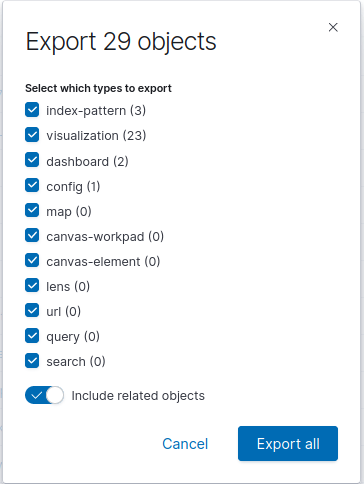
\includegraphics[width=5cm, keepaspectratio]{img/export_kibana.png}
			\caption{Exportación en interfaz Kibana.}
			\label{fig:export_kibana}
		\end{figure}
		
		Esta herramienta genera un fichero \texttt{NDJSON} similar a la estructura \texttt{JSON} con los patrones de índices creados, así como las visualizaciones, tablas o \textit{scripted fields} guardados en Kibana.\\
		
		Para que un futuro desarrollador importe estos datos simplemente podrá hacerlo por la interfaz gráfica de Kibana. Para unificar la metodología y ya que en el servidor de pre-producción/producción no se dispone de esta interfaz gráfica, esta también se puede realizar mediante la siguiente sentencia:\\
		
		
		{\footnotesize
		\begin{verbatim}
			$ curl -X POST "localhost:5601/api/saved_objects/_import" -H "kbn-xsrf: true" 
			--form file=@kibotics_dummy_kibana.ndjson
		\end{verbatim}
		}


	\cleardoublepage 
	\chapter{Conclusiones} 
	\label{chap:conclusiones} 
		Finalmente, en este último capítulo se exponen las conclusiones alcanzadas, así como las competencias adquiridas durante la realización de este proyecto. Además, se plantean futuros trabajos de ampliación y mejora sobre el software desarrollado.
	
	\section{Conclusiones finales} 
	\label{sec:conclusiones_finales} 

		Repasando lo plateado en el capítulo \ref{chap:objetivos}, el objetivo de este proyecto es crear una herramienta con la que grabar datos de actividad, visualizar y analizar el uso que hacen los usuarios de la plataforma educativa Kibotics. Este objetivo global se ha cumplido satisfactoriamente: se ha diseñado, desarrollado y probado un módulo de analíticas en el que visualizar estos datos de uso de la aplicación.\\
		
		La herramienta desarrollada consta de la grabación de un conjunto más extenso de eventos de los que poseía inicialmente y una vista específica, llamada 'Analíticas' dentro del servidor web de Kibotics. Esta nueva vista tiene embebida los tableros o \textit{dashboards} que se generan en el servicio de Kibana.\\
		
		Se ha mejorado el sistema de registro de logs de la aplicación como se explicó en la Subsección \ref{subsec:elasticsearch_kibotics}, ampliando y extendiendo el conjunto de sondas que graban eventos de interés. Eliminando los ficheros de log indexados por días y creando una base de datos en Elasticsearch dividida en distintos índices sobre los que se registran variedad de eventos interesantes como inicio de sesión, entrada en cada ejercicio, desde qué sistema operativo se accede a la plataforma, etc... Aumentando así la escalabilidad de este proceso de registro de logs y eventos, con este cambio se consigue que esta sea una solución robusta y duradera.\\
	
		Se ha desarrollado una vista en la web de Kibotics en la que se muestran automáticamente los datos agregados que están almacenados en la base de datos, detallado en la Subsección \ref{subsec:kibana_kibotics}. Es una vista dinámica, con los contenidos que se muestran generados en caliente, en ese mismo momento, desde los datos almacenados. Eso permite una visualización siempre actualizada. En esta vista de Django se muestran varios cortes del conjunto de datos como la ubicación geográfica desde donde se accede a la plataforma, la frecuencia y duración de las interacciones de los usuarios con la plataforma a lo largo del tiempo. \\
	
		Además de las tecnologías empleadas en el segundo prototipo (Elasticsearch y Kibana), se han explorado otras opciones. En el campo de las bases de datos se hizo uso de MongoDB como soporte para toda la información circunstancial que posteriormente se visualizaba haciendo uso de la librería de Python Matplotlib, según se explica con detalle en el capítulo \ref{chap:primer_prototipo} \\

		
		\begin{table}[H]
			\begin{center}
				\begin{tabular}{ | c | p{6cm} | c | c |} 
					\hline
				 & Eventos registrados & Almacenamiento & Visualización \\ 
					\hline 
					Kibotics 2.0 & Inicio de sesión, fin de sesión, comienzo de ejercicio, salida de ejercicio y error en aplicación & Ficheros TXT & No\\ 
					\hline
					Primer Prototipo & Inicio de sesión, fin de sesión, comienzo de ejercicio, salida de ejercicio y error en aplicación& MongoBD 4.2.6 & Matplotlib 3.1.2\\ 
					\hline
					Segundo Prototipo & Sesión unificado y enriquecido, simulación  unificado y enriquecido, visitantes y error en aplicación & Elasticsearch 7.6.2 & Kibana 7.7.0\\ 
					\hline

				\end{tabular}
				\label{tabla:evolucion_analiticas}
				\caption{Evolución del sistema de registro de eventos y analíticas de la plataforma educativa Kibotics.}
			\end{center}
		\end{table}
	
				
		En la Tabla \ref{tabla:evolucion_analiticas} se puede observar de forma esquemática la evolución que han sufrido las sondas de datos circunstanciales, así como las tecnologías de bases de datos y de visualización utilizadas en el desarrollo de este Trabajo Fin de Grado.
	\section{Competencias adquiridas} 
	\label{sec:competencias_adquiridas} 
	
		En esta sección se enumeran las principales habilidades que se han adquirido en el desarrollo de este proyecto:
		\begin{itemize}
			\item Django y Python como herramientas muy potentes y accesibles para el desarrollo Web. Además, gracias a las librerías de las que estas disponen, son herramientas muy versátiles.\\
			
			\item Despliegue e implementación de diferentes tipos de bases de datos MongoDB y Elasticsearch en un proyecto real. Importancia de la información para monitorizar un servicio Web.\\
			
			\item Se han explorado dos tecnologías diferentes para la visualización automática de información. Primero la librería de Python Matplotlib, que pese a las limitaciones encontradas, ofrece una gran versatilidad. Y finalmente Kibana, que gracias al stack ELK proporciona un ecosistema rápido, potente y escalable con el que trabajar. \\
			
			\item Una primera toma en contacto con el análisis web automático en el que ha destacado el uso del stack ELK. Este ha sido una herramienta muy potente de la que he aprendido cómo es integrar varias tecnologías para crear un producto complejo, interconectado e interesante. \\
			
			
			\item Sistema de versiones centrado en los parches e incidencias. Haciendo uso de GitHub como repositorio en el que desarrollar este Trabajo Fin de Grado, siempre presente junto a la filosofía \textit{release often, release soon}. \\
			
			\item Trabajar en un software complejo y actualmente en producción sobre el que desarrollar para crear nuevas funcionalidades y sobre el que trabaja un equipo con el que es necesario estar el sincronía para realizar las integraciones de los parches. \\
			
		\end{itemize}
	\section{Trabajos futuros} 
	\label{sec:trabajos_futuros} 

		En esta sección se proponen una serie de mejoras o ampliaciones con las que aumentar la funcionalidad del módulo de analíticas desarrollado:

		\begin{itemize}
			\item Kibotics Webserver es una aplicación grande y en constante ampliación, añadir más sondas con las que tener la aplicación controlada será recomendable. Con estas nuevas sondas será necesaria la creación de nuevos índices en la base de datos y visualizaciones automáticas en la vista de analíticas.\\
			
			\item Actualmente los datos almacenados en Elasticsearch solo pueden ser analizados accediendo al módulo desarrollado. Una nueva herramienta automática externa que analice estos datos sería muy interesante para monitorizar, por ejemplo, que todos los ejercicios están siendo accedidos y los tiempos de desarrollo de los usuarios no son demasiado elevados.\\
			
			\item El stack ELK posee, además de Elasticsearch y Kibana, otras herramientas muy interesantes como Logstash y Beats. Ellas pueden dotar a Elasticsearch de nuevos datos procedentes de otras fuentes, como por ejemplo logs del servidor con los que controlar los accesos que recibe la plataforma y el servidor Apache subyacente. \\
			
			\item Explorar otras mejoras de integración en la plataforma de Kibotics, ya que el iframe no es algo ideal en un servicio en producción, principalmente por motivos de seguridad. Buscar otras configuraciones de Kibana que permitan un mejor despliegue en los servicios de \textit{Amazon Web Service} desde los que se ejecuta la plataforma.\\
						
			\item Al proporcionar información muy sensible sobre el servicio de la plataforma, es necesario aumentar la seguridad en el servidor Kibotics para acceder a las vistas en las que se visualizan estos datos.\\
		\end{itemize}


	\cleardoublepage
	\begin{thebibliography}{7}
		
		\bibitem{SVod}
		\textit{Mercado video on demand:}
		\url{https://www.merca20.com/infografia-asi-es-el-mercado-del-video-on-demand/}
		
		\bibitem{HTML}
		\textit{Estándar HTML:}
		\url{https://html.spec.whatwg.org/}
		
		\bibitem{JavaScript}
		\textit{Documentación JavaScript MDN web docs:}
		\url{https://developer.mozilla.org/es/docs/Web/JavaScript}	
		
		\bibitem{Django MVC}
		\textit{Patrón Django Model-View-Controller:}
		\url{https://uniwebsidad.com/libros/django-1-0/capitulo-5/el-patron-de-diseno-mtv}
		
		\bibitem{Django}
		\textit{Documentación \textit{Django Project}:}
		\url{https://www.djangoproject.com/}
		
		\bibitem{MongoDB}
		\textit{Documentación MongoDB:}
		\url{https://docs.mongodb.com/guides/server/introduction/}	
		
		\bibitem{Use_MongoDB}
		\textit{Quíen usa MongoDB:}
		\url{https://www.mongodb.com/who-uses-mongodb}
		
		\bibitem{elasticsearch}
		\textit{Documentación Elasticsearch:}
		\url{https://www.elastic.co/guide/en/elasticsearch/reference/current/index.html}
		
		\bibitem{versions_elasticsearch}
		\textit{Histórico de versiones para Elasticsearch:}
		\url{https://www.elastic.co/downloads/past-releases#elasticsearch}	
		
		\bibitem{releases_matplotlib}
		\textit{Versiones de Matplotlib:}
		\url{https://github.com/matplotlib/matplotlib/releases}	
		
		\bibitem{kibana}
		\textit{Documentación Kibana:}
		\url{https://www.elastic.co/guide/en/kibana/current/index.html}	
		
		\bibitem{versions_kibana}
		\textit{Histórico de versiones para Kibana:}
		\url{https://www.elastic.co/downloads/past-releases#kibana}	
		
		\bibitem{Matplotlib}
		\textit{Documentación Matplotlib:}
		\url{https://matplotlib.org/}
		
		\bibitem{Elasticdump}
		\textit{Documentación Elasticdump:}
		\url{https://www.npmjs.com/package/elasticdump}	

	\end{thebibliography}
	
\end{document}